%---------------------------------------------------------------------------%
%-                                                                         -%
%-                           LaTeX Template                                -%
%-                                                                         -%
%---------------------------------------------------------------------------%
%- Copyright (C) Huangrui Mo <huangrui.mo@gmail.com> 
%- This is free software: you can redistribute it and/or modify it
%- under the terms of the GNU General Public License as published by
%- the Free Software Foundation, either version 3 of the License, or
%- (at your option) any later version.
%---------------------------------------------------------------------------%
%->> Document class declaration
%---------------------------------------------------------------------------%
\documentclass[print]{Style/ucasthesis}%
%- Multiple optional arguments:
%- [<oneside|twoside|print>]% oneside eprint, twoside eprint, or paper print
%- [fontset=<adobe|none|...>]% specify font set instead of automatic detection
%- [scheme=plain]% thesis writing of international students
%- [draftversion]% show draft version information
%- [standard options for ctex book class: draft|paper size|font size|...]%
%---------------------------------------------------------------------------%
%->> Document settings
%---------------------------------------------------------------------------%
\usepackage[super, geometry, list]{Style/artratex}% document settings
%- usage: \usepackage[option1,option2,...,optionN]{artratex}
%- Multiple optional arguments:
%- [bibtex|biber]% set bibliography processor and package
%- [<numbers|super|authoryear|alpha>]% set citation and reference style
%- <numbers>: textual: Jones [1]; parenthetical: [1]
%- <super>: textual: Jones superscript [1]; parenthetical: superscript [1]
%- <authoryear>: textual: Jones (1995); parenthetical: (Jones, 1995)
%- <alpha>: textual: not available; parenthetical: [Jon95]
%- [geometry]% reconfigure page layout via geometry package
%- [lscape]% provide landscape layout environment
%- [xhf]% disable header and footer via fancyhdr package
%- [color]% provide color support via xcolor package
%- [background]% enable page background
%- [tikz]% provide complex diagrams via tikz package
%- [table]% provide complex tables via ctable package
%- [list]% provide enhanced list environments for algorithm and coding
%- [math]% enable some extra math packages
%- [xlink]% disable link colors
\usepackage{Style/artracom}% user defined commands
%---------------------------------------------------------------------------%
%->> Document inclusion
%---------------------------------------------------------------------------%
%\includeonly{Tex/Chap_1,...,Tex/Chap_N}% selected files compilation
%---------------------------------------------------------------------------%
%->> Document content
%---------------------------------------------------------------------------%
%-
%-> Titlepage information
%-
%---------------------------------------------------------------------------%
%->> Titlepage information
%---------------------------------------------------------------------------%
%-
%-> 中文封面信息
%-
% \confidential{}% 密级:只有涉密论文才填写
% \schoollogo[scale=0.095]{ucas_logo}% 校徽
\title{深度神经网络硬件加速系统设计与优化}% 论文中文题目
\author{王磊}% 论文作者
\advisor{朱艾春\\}% 指导教师:姓名 专业技术职务 工作单位
%\advisor{指导教师一\\指导教师二\\指导教师三}% 多行指导教师示例
\degree{学士}% 学位:学士、硕士、博士
\degreetype{理学}% 学位类别:理学、工学、工程、医学等
\major{电子信息工程}% 二级学科专业名称
% \institute{中国科学院力学研究所}% 院系名称
%\institute{中国科学院力学研究所\\流固耦合实验室}% 多行院系名称示例
\date{2014~年~6~月}% 毕业日期:夏季为6月、冬季为12月
%-
%-> 英文封面信息
%-
\TITLE{\LaTeX{} Thesis Template\\ of \\ The University of Chinese Academy of Sciences {$~^{\pi}\pi^{\pi}$}}% 论文英文题目
\AUTHOR{Mo Huangrui}% 论文作者
\ADVISOR{Supervisor: Professor Liu Qingquan}% 指导教师
\DEGREE{Master}% 学位:Bachelor, Master, Doctor, Postdoctor。封面据英文学位名称自动切换,需确保拼写准确
\DEGREETYPE{Natural Science}% 学位类别:Philosophy, Natural Science, Engineering, Economics, Agriculture 等
\MAJOR{Fluid Mechanics}% 二级学科专业名称
\INSTITUTE{Institute of Mechanics, Chinese Academy of Sciences}% 院系名称
\DATE{June, 2014}% 毕业日期:夏季为June、冬季为December
%---------------------------------------------------------------------------%
%
\begin{document}
\nocite{*}
%-
%-> Frontmatter: title page, abstract, content list, symbol list, preface
%-
\frontmatter% initialize the environment
%---------------------------------------------------------------------------%
%->> Frontmatter
%---------------------------------------------------------------------------%
%-
%-> 生成封面
%-
\maketitle% 生成中文封面
% \MAKETITLE% 生成英文封面
%-
%-> 作者声明
%-
% \makedeclaration% 生成声明页
%-
%-> 中文摘要
%-
% \intobmk\chapter*{摘要}% 显示在书签但不显示在目录
% syntax: \chapter[目录]{标题}\chaptermark{页眉}
\chapter[摘要]{\MyTitleCh}\chaptermark{摘要}
\setcounter{page}{1}% 开始页码
\pagenumbering{Roman}% 页码符号

\begin{center}
\vspace{-0.3cm}
\zihao{3} \songti 摘要
\vspace{0.3cm}
\end{center}

近年来,深度神经网络已经被证明在包括图像分类、目标检测和自然语言处理等任务上能够取得相当不错的效果。现如今,大量的应用程序都配备了与之相关的深度学习算法,但是对于手机、无人机等资源有限的嵌入式设备上,仅用软件方式加速深度神经网络已经不能满足日益增长的速度和功耗要求,如何利用硬件设计加速器已经成为学术领域的研究热点。

本文首先给出了深度神经网络的概述,并介绍了几种当下主流的针对深度神经网络的硬件加速系统设计方案以及实际应用。在硬件设计方面,本设计主要基于 ZYNQ 7000 器件将英伟达开源的 NVDLA 框架在 FPGA 侧进行了实现与评估,并将其通过 AXI4 总线挂载到双核的 ARM A9 处理器上。软件设计层面,在服务器端,使用 Caffe 框架针对 MNIST、CIFAR10、IMAGENET 训练了三个有精度的分类模型,并结合 TensorRT 进行了 INT8 量化;在主机端,编译神经网络编译器接受训练好的模型生成序列化数据流文件;在硬件端,本设计为 ARM A9 处理器移植了 Ubuntu 操作系统,将硬件加速器的驱动程序挂载到 Linux 内核,通过运行时调度硬件加速器进行推理,分析了该过程中的精度损失情况、与CPU相比的运行速度差异,并分析了原因。

{
    \zihao{5}
    \keywords{深度神经网络 \quad FPGA \quad NVDLA \quad 硬件加速}% 中文关键词
}
%-
%-> 英文摘要
%-
% \intobmk\chapter*{Abstract}% 显示在书签但不显示在目录
\chapter[Abstract]{\MyTitleEn}\chaptermark{Abstract}

\begin{center}
\vspace{-0.3cm}
\zihao{3} \songti Abstract
\vspace{0.3cm}
\end{center}

In recent years, deep neural networks have been proven to achieve quite good results in tasks including image classification, target detection, and natural language processing. Nowadays, a large number of applications are equipped with related deep learning algorithms. However, for embedded devices with limited resources such as mobile phones and drones, the use of software to accelerate deep neural networks can no longer meet the increasing speed and Power consumption requirements, how to use hardware design accelerators have become a research hotspot in the academic field.

This article first gives an overview of deep neural networks, and introduces several current mainstream hardware acceleration system design schemes and practical applications for deep neural networks. In terms of hardware design, this design is mainly based on the ZYNQ 7000 device to implement and evaluate Nvidia's open source NVDLA framework on the FPGA side, and mount it to the dual-core ARM A9 processor through the AXI4 bus. At the software design level, on the server side, the Caffe framework is used to train three accurate classification models for MNIST, CIFAR10, and IMAGENET, and combined with TensorRT for INT8 quantization; on the host side, the neural network compiler is compiled to receive the trained model generation Serialized data stream files; on the hardware side, this design transplants the Ubuntu operating system to the ARM A9 processor, mounts the driver of the hardware accelerator to the Linux kernel, and schedules the hardware accelerator at runtime for reasoning, and analyzes the process of The loss of accuracy, the difference in operating speed compared with the CPU, and the reasons are analyzed.

\KEYWORDS{Deep neural network; FPGA; NVDLA; Hardware speedup}% 英文关键词
%---------------------------------------------------------------------------%
% title page, abstract
{% content list region
\linespread{1.2}% local line space
\intobmk*{\cleardoublepage}{\contentsname}% add link to bookmark
\tableofcontents% content catalog
% \intobmk*{\cleardoublepage}{\listfigurename}% add link to bookmark
% \listoffigures% figure catalog
% \intobmk*{\cleardoublepage}{\listtablename}% add link to bookmark
% \listoftables% table catalog
}
% \intobmk\chapter*{符号列表}% 显示在书签但不显示在目录

\section*{字符}
\nomenclatureitem[\textbf{Unit}]{\textbf{Symbol}}{\textbf{Description}}
\nomenclatureitem[$\Unit{m^{2} \cdot s^{-2} \cdot K^{-1}}$]{$R$}{the gas constant}
\nomenclatureitem[$\Unit{m^{2} \cdot s^{-2} \cdot K^{-1}}$]{$C_v$}{specific heat capacity at constant volume}
\nomenclatureitem[$\Unit{m^{2} \cdot s^{-2} \cdot K^{-1}}$]{$C_p$}{specific heat capacity at constant pressure}
\nomenclatureitem[$\Unit{m^{2} \cdot s^{-2}}$]{$E$}{specific total energy}
\nomenclatureitem[$\Unit{m^{2} \cdot s^{-2}}$]{$e$}{specific internal energy}
\nomenclatureitem[$\Unit{m^{2} \cdot s^{-2}}$]{$h_T$}{specific total enthalpy}
\nomenclatureitem[$\Unit{m^{2} \cdot s^{-2}}$]{$h$}{specific enthalpy}
\nomenclatureitem[$\Unit{kg \cdot m \cdot s^{-3} \cdot K^{-1}}$]{$k$}{thermal conductivity}
\nomenclatureitem[$\Unit{kg \cdot m^{-1} \cdot s^{-2}}$]{$S_{ij}$}{deviatoric stress tensor}
\nomenclatureitem[$\Unit{kg \cdot m^{-1} \cdot s^{-2}}$]{$\tau_{ij}$}{viscous stress tensor}
\nomenclatureitem[$\Unit{1}$]{$\delta_{ij}$}{Kronecker tensor}
\nomenclatureitem[$\Unit{1}$]{$I_{ij}$}{identity tensor}

\section*{算子}
\nomenclatureitem{\textbf{Symbol}}{\textbf{Description}}
\nomenclatureitem{$\Delta$}{difference}
\nomenclatureitem{$\nabla$}{gradient operator}
\nomenclatureitem{$\delta^{\pm}$}{upwind-biased interpolation scheme}

\section*{缩写}
\nomenclatureitem{CFD}{Computational Fluid Dynamics}
\nomenclatureitem{CFL}{Courant-Friedrichs-Lewy}
\nomenclatureitem{EOS}{Equation of State}
\nomenclatureitem{JWL}{Jones-Wilkins-Lee}
\nomenclatureitem{WENO}{Weighted Essentially Non-oscillatory}
\nomenclatureitem{ZND}{Zel'dovich-von Neumann-Doering}

% symbol list, preface content
%-
%-> Mainmatter
%-
\mainmatter% initialize the environment
%---------------------------------------------------------------------------%
%->> Main content
%---------------------------------------------------------------------------%
\chapter{引言}\label{chap:introduction}

\section{研究背景}

考虑到许多同学可能缺乏\LaTeX{}使用经验,ucasthesis将\LaTeX{}的复杂性高度封装,开放出简单的接口,以便轻易使用。同时,对用\LaTeX{}撰写论文的一些主要难题,如制图、制表、文献索引等,进行了详细说明,并提供了相应的代码样本,理解了上述问题后,对于初学者而言,使用此模板撰写学位论文将不存在实质性的困难。所以,如果你是初学者,请不要直接放弃,因为同样为初学者的我,十分明白让\LaTeX{}简单易用的重要性,而这正是ucasthesis所追求和体现的。

此中国科学院大学学位论文模板ucasthesis基于中科院数学与系统科学研究院吴凌云研究员的CASthesis模板发展而来。当前ucasthesis模板满足最新的中国科学院大学学位论文撰写要求和封面设定。兼顾操作系统:Windows,Linux,MacOS 和\LaTeX{}编译引擎:pdflatex,xelatex,lualatex。支持中文书签、中文渲染、中文粗体显示、拷贝PDF中的文本到其他文本编辑器等特性。此外,对模板的文档结构进行了精心设计,撰写了编译脚本提高模板的易用性和使用效率。

ucasthesis的目标在于简化学位论文的撰写,利用\LaTeX{}格式与内容分离的特征,模板将格式设计好后,作者可只需关注论文内容。 同时,ucasthesis有着整洁一致的代码结构和扼要的注解,对文档的仔细阅读可为初学者提供一个学习\LaTeX{}的窗口。此外,模板的架构十分注重通用性,事实上,ucasthesis不仅是国科大学位论文模板,同时,通过少量修改即可成为使用\LaTeX{}撰写中英文文章或书籍的通用模板,并为使用者的个性化设定提供了接口。

\section{系统要求}\label{sec:system}

\href{https://github.com/mohuangrui/ucasthesis}{\texttt{ucasthesis}} 宏包可以在目前主流的 \href{https://en.wikibooks.org/wiki/LaTeX/Introduction}{\LaTeX{}} 编译系统中使用,如\TeX{}Live和MiK\TeX{}。因C\TeX{}套装已停止维护,\textbf{不再建议使用} (请勿混淆C\TeX{}套装与ctex宏包。C\TeX{}套装是集成了许多\LaTeX{}组件的\LaTeX{}编译系统。 \href{https://ctan.org/pkg/ctex?lang=en}{ctex} 宏包如同ucasthesis,是\LaTeX{}命令集,其维护状态活跃,并被主流的\LaTeX{}编译系统默认集成,是几乎所有\LaTeX{}中文文档的核心架构)。推荐的 \href{https://en.wikibooks.org/wiki/LaTeX/Installation}{\LaTeX{}编译系统} 和 \href{https://en.wikibooks.org/wiki/LaTeX/Installation}{\LaTeX{}文本编辑器} 为
\begin{center}
    %\footnotesize% fontsize
    %\setlength{\tabcolsep}{4pt}% column separation
    %\renewcommand{\arraystretch}{1.5}% row space 
    \begin{tabular}{lcc}
        \hline
        %\multicolumn{num_of_cols_to_merge}{alignment}{contents} \\
        %\cline{i-j}% partial hline from column i to column j
        操作系统 & \LaTeX{}编译系统 & \LaTeX{}文本编辑器\\
        \hline
        Linux & \href{https://www.tug.org/texlive/acquire-netinstall.html}{\TeX{}Live Full} & \href{http://www.xm1math.net/texmaker/}{Texmaker} 或 Vim\\
        MacOS & \href{https://www.tug.org/mactex/}{Mac\TeX{} Full} & \href{http://www.xm1math.net/texmaker/}{Texmaker} 或 Texshop\\
        Windows & \href{https://www.tug.org/texlive/acquire-netinstall.html}{\TeX{}Live Full} 或 \href{https://miktex.org/download}{MiK\TeX{}} & \href{http://www.xm1math.net/texmaker/}{Texmaker}\\
        \hline
    \end{tabular}
\end{center}

\LaTeX{}编译系统,如\TeX{}Live(Mac\TeX{}为针对MacOS的\TeX{}Live),用于提供编译环境,\LaTeX{}文本编辑器 (如Texmaker) 用于编辑\TeX{}源文件。请从各软件官网下载安装程序,勿使用不明程序源。\textbf{\LaTeX{}编译系统和\LaTeX{}编辑器分别安装成功后,即完成了\LaTeX{}的系统配置},无需其他手动干预和配置。若系统原带有旧版的\LaTeX{}编译系统并想安装新版,请\textbf{先卸载干净旧版再安装新版}。

\section{问题反馈}

请见 \href{https://github.com/mohuangrui/ucasthesis/wiki/%E5%B8%B8%E8%A7%81%E9%97%AE%E9%A2%98}{问题反馈} 

欢迎大家有效地反馈模板不足之处,一起不断改进模板。希望大家向同事积极推广\LaTeX{},一起更高效地做科研。

\section{模板下载}

\begin{center}
    \href{https://github.com/mohuangrui/ucasthesis}{Github/ucasthesis}: \url{https://github.com/mohuangrui/ucasthesis}
\end{center}

\chapter{相关技术介绍}\label{chap:relate}

由于本系统涉及软硬件协同设计,在进行设计前需要对神经网络算法、RISC-V 处理器以及 FPGA 平台有足够的认识。在本系统的设计中,我们需要选择合适的神经网络算法,并对其进行硬件加速。由于不是所有的运算都适合放在 FPGA 上实现,同时也为了加速器通用性的考虑,本设计中还使用一个 RISC-V 处理器来分担一部分运算任务以及流程控制的工作。

\section{神经网络概述}

\subsection{卷积神经网络概述}

\begin{figure}[!htbp]
    \centering
    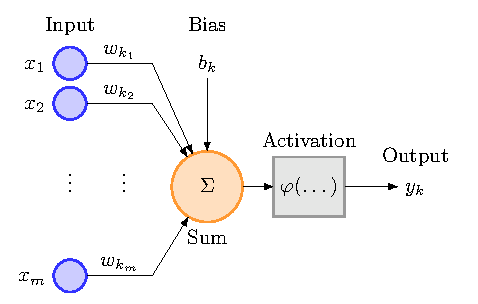
\includegraphics[width=0.5\textwidth]{neuron}
    \caption{神经元模型}
    \label{fig:neuron}
\end{figure}

一个神经元模型由输入信号、权值、偏置、加法器和激活函数共同构成,如图~\ref{fig:neuron}所示,每个神经元都是一个多输入单输出的信息处理单元,其中 $w_{kj}$ 下标的含义为:$k$ 表示第 $k$ 个神经元;$j$ 表示第 $j$ 个输入。因此,$w_{kj}$表示第 $k$ 个神经元的第 $j$ 个输入对应的权值。单个神经元的数学公式如公式~\eqref{eq:neuron} 所示:
\begin{equation} \label{eq:neuron}
% \adddotsbeforeeqnnum%
\begin{cases}
u_k = \sum_{j=1}^{m} w_{kj}x_j & \\
v_k = u_k + b_k & \\
y_k = \varphi(v_k) &
\end{cases}
\end{equation}

其中 $x_j$ 表示第 $k$ 个神经元的第 $j$ 个输入,$w_{kj}$表示第 $k$ 个神经元的第 $j$ 个输入对应的权值,$b_k$ 表示第 $k$ 个神经元的偏置,$\varphi(\dots)$ 为激活函数,$y_k$ 为该神经元的输出。前两个表达式为线性运算,而激活函数为非线性运算,因此通过激活函数向神经网络中引入非线性因素,使得神经网络几乎可以逼近任意函数。

\begin{figure}[!htbp]
    \centering
    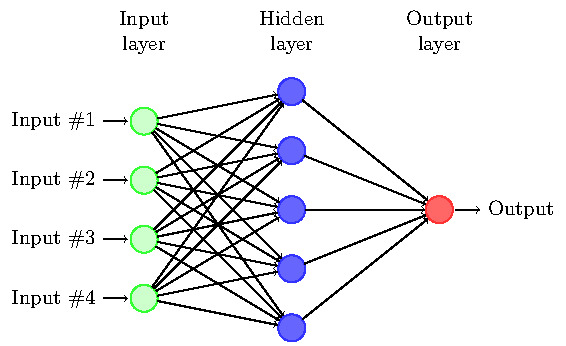
\includegraphics[width=0.6\textwidth]{FNN}
    \caption{前向神经网络结构}
    \label{fig:FNN}
\end{figure}

将多个神经元按层排列,各层之间前后级联,就组成了前向神经网络(Feedforward neural network, FNN),其结构如图~\ref{fig:FNN}所示。前向神经网络通常包含了输入层、隐藏层和输出层。

卷积神经网络(Convolutional Neural Network, CNN)是目前最常用的一种前向神经网络,对于大型图像处理有出色表现。一个典型的卷积神经网络结构(LeNet-5)\citep{lecun1998gradient} 如图~\ref{fig:CNN}所示:

\begin{figure}[!htbp]
    \centering
    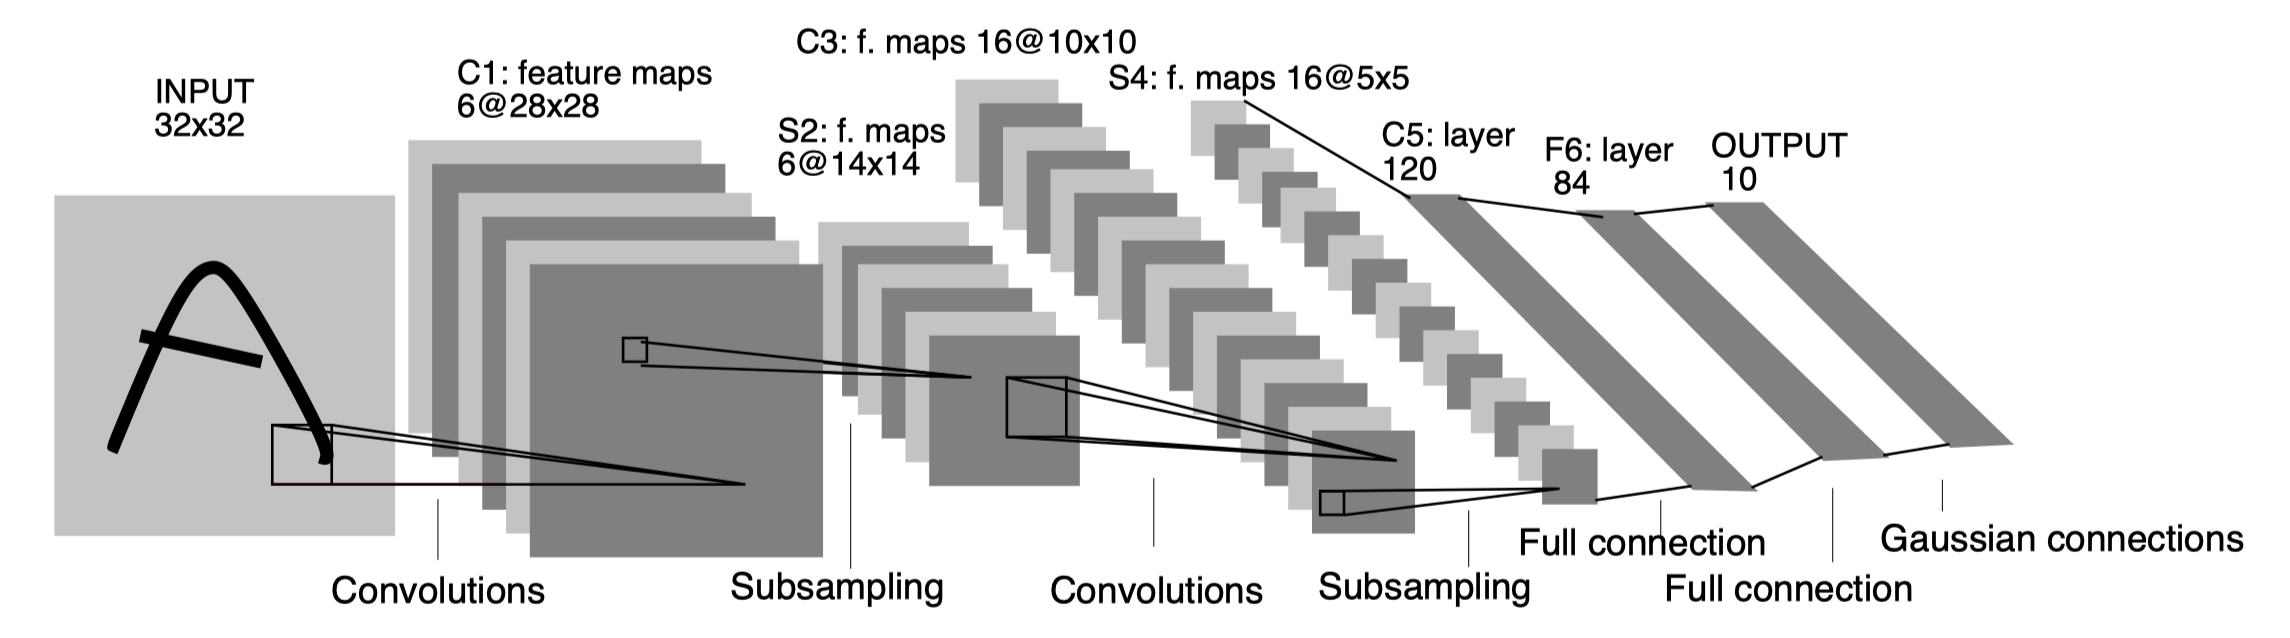
\includegraphics[width=0.9\textwidth]{CNN}
    \caption{LeNet-5 \ 网络结构}
    \label{fig:CNN}
\end{figure}

输入为一幅手写字母的图像,经过卷积神经网络的运算后,输出识别的结果。卷积神经网络主要包含了卷积层、池化层和全连接层 3 种结构,卷积层主要用来提取图像中的局部特征,池化层用来降低参数数量级,全连接层类似于卷积层,用来输出结果。

\subsection{YOLO 算法介绍}

YOLO 算法\citep{redmon2016you}于2016由 Joseph Redmon 等人提出,YOLO 的全称是 you only look once,指只需要浏览一次就可以识别出图像中物体的类别和位置。相比于 Region-based 的两阶段(2-stage)方式,YOLO 的单阶段(1-stage)扫描方式更适合通过流水线优化的方法进行硬件加速。YOLO 算法目前已经发展到了第四代,但是由于 YOLO V3 和 YOLO V4 引入了残差模型和FPN架构等新结构,使得整个神经网络结构更深,从 YOLO V2 的 darknet-19\citep{redmon2017yolo9000} 到 YOLO V3 的 darknet-53\citep{redmon2018yolov3},通过硬件加速需要消耗更多的资源,在低成本的 FPGA 芯片上难以实现,因此本文选用了 YOLO V2 算法作为硬件加速的对象。

TINY YOLO 算法是 YOLO 算法的简化版,在牺牲一定精度的代价下,其速度得到了大幅提高,且结构更加精简,适得其更加适合在硬件资源极度有限的低成本 FPGA 上实现。TINY YOLO 算法与 YOLO 算法的对比见表~\ref{tab:tiny},可以看到,对比原版 YOLO 算法,TINY YOLO 算法在准确度上有小幅度下降,但是其速度极快,最快达到了 207 FPS。

\begin{table}[!htbp]
\caption{TINY YOLO 与 YOLO 对比}
\label{tab:tiny}
\centering
\footnotesize% fontsize
\setlength{\tabcolsep}{4pt}% column separation
\renewcommand{\arraystretch}{1.2}%row space 
\begin{tabular}{lccccc}
\toprule
Model & Train & Test & mAP & FLOPS & FPS \\
\midrule
YOLOv2 & VOC 2007+2012 & 2007 & 76.8 & 34.90 Bn & 67 \\
YOLOv2 544x544 & VOC 2007+2012 & 2007 & 78.6 & 59.68 Bn & 40 \\
Tiny YOLO & VOC 2007+2012 & 2007 & 57.1 & 6.97 Bn & 207 \\
\bottomrule
\end{tabular}
\end{table}

YOLO V2 算法的结构如表~\ref{tab:darknet19}所示,其包含了19个卷积层,5个最大池化层以及一个全连接层。

% \begin{figure}[!htbp]
%     \centering
%     \includegraphics[height=0.70\textheight]{yolov2-tiny-structure}
%     \caption{TINY YOLO 网络结构}
%     \label{fig:yolov2-tiny-structure}
% \end{figure}


% \begin{table}[!htbp]
% \caption{Darknet-19}
% \label{tab:darknet19}
% \centering
% \footnotesize% fontsize
% \setlength{\tabcolsep}{4pt}% column separation
% \renewcommand{\arraystretch}{1.0}%row space 
% \begin{tabular}{c|c|c|c}
% \toprule
% Type & Filters & Size/Stride & Output \\
% \midrule
% Convolutional & 32   & 3 × 3   & 224 × 224 \\
% Maxpool       &      & 2 × 2/2 & 112 × 112 \\
% Convolutional & 64   & 3 × 3   & 112 × 112 \\
% Maxpool       &      & 2 × 2/2 & 56 × 56 \\
% Convolutional & 128  & 3 × 3   & 56 × 56 \\
% Convolutional & 64   & 1 × 1   & 56 × 56 \\
% Convolutional & 128  & 3 × 3   & 56 × 56 \\
% Maxpool       &      & 2 × 2/2 & 28 × 28 \\
% Convolutional & 256  & 3 × 3   & 28 × 28 \\
% Convolutional & 128  & 1 × 1   & 28 × 28 \\
% Convolutional & 256  & 3 × 3   & 28 × 28 \\
% Maxpool       &      & 2 × 2/2 & 14 × 14 \\
% Convolutional & 512  & 3 × 3   & 14 × 14 \\
% Convolutional & 256  & 1 × 1   & 14 × 14 \\
% Convolutional & 512  & 3 × 3   & 14 × 14 \\
% Convolutional & 256  & 1 × 1   & 14 × 14 \\
% Convolutional & 512  & 3 × 3   & 14 × 14 \\
% Maxpool       &      & 2 × 2/2 & 7 × 7 \\
% Convolutional & 1024 & 3 × 3   & 7 × 7 \\
% Convolutional & 512  & 1 × 1   & 7 × 7 \\
% Convolutional & 1024 & 3 × 3   & 7 × 7 \\
% Convolutional & 512  & 1 × 1   & 7 × 7 \\
% Convolutional & 1024 & 3 × 3   & 7 × 7 \\
% \midrule

% Convolutional & 1000 & 1 × 1   & 7 × 7 \\
% Avgpool       &      & Global  & 1000 \\
% Softmax       &      &         &      \\
% \bottomrule
% \end{tabular}
% \end{table}

{
\zihao{-5}
% Change the intercolumn space
\setlength{\tabcolsep}{10pt}

\begin{longtable}{cccc}
    \caption{Darknet-19 网络结构} \label{tab:darknet19}\\

    % Appear table header at the first page as well
    \toprule
    Type & Filters & Size/Stride & Output \\
    \midrule
    \endfirsthead

    \multicolumn{4}{c}%
    {\bfseries\small \tablename\ \thetable\ {续表}}\\

    % Appear the table header at the top of every page
    \toprule
    Type & Filters & Size/Stride & Output \\
    \midrule
    \endhead

    \midrule \multicolumn{4}{r}{\textit{续表见下页}}\\
    \endfoot

     % Appear \hline at the bottom of every page
    \bottomrule
    \endlastfoot

    Convolutional & 32   & 3 × 3   & 224 × 224 \\
    Maxpool       &      & 2 × 2/2 & 112 × 112 \\
    Convolutional & 64   & 3 × 3   & 112 × 112 \\
    Maxpool       &      & 2 × 2/2 & 56 × 56 \\
    Convolutional & 128  & 3 × 3   & 56 × 56 \\
    Convolutional & 64   & 1 × 1   & 56 × 56 \\
    Convolutional & 128  & 3 × 3   & 56 × 56 \\
    Maxpool       &      & 2 × 2/2 & 28 × 28 \\
    Convolutional & 256  & 3 × 3   & 28 × 28 \\
    Convolutional & 128  & 1 × 1   & 28 × 28 \\
    Convolutional & 256  & 3 × 3   & 28 × 28 \\
    Maxpool       &      & 2 × 2/2 & 14 × 14 \\
    Convolutional & 512  & 3 × 3   & 14 × 14 \\
    Convolutional & 256  & 1 × 1   & 14 × 14 \\
    Convolutional & 512  & 3 × 3   & 14 × 14 \\
    Convolutional & 256  & 1 × 1   & 14 × 14 \\
    Convolutional & 512  & 3 × 3   & 14 × 14 \\
    Maxpool       &      & 2 × 2/2 & 7 × 7 \\
    Convolutional & 1024 & 3 × 3   & 7 × 7 \\
    Convolutional & 512  & 1 × 1   & 7 × 7 \\
    Convolutional & 1024 & 3 × 3   & 7 × 7 \\
    Convolutional & 512  & 1 × 1   & 7 × 7 \\
    Convolutional & 1024 & 3 × 3   & 7 × 7 \\
    \midrule

    Convolutional & 1000 & 1 × 1   & 7 × 7 \\
    Avgpool       &      & Global  & 1000 \\
    Softmax       &      &         &      \\
\end{longtable}
}

根据 YOLO 论文\citep{redmon2016you,redmon2017yolo9000,redmon2018yolov3}及 Darknet 网络源码分析 YOLO V2 进行目标检测的步骤如下:

\begin{enumerate}
\item 首先输入任意尺寸的 RGB 格式的图像,将各像素的值归一化到0-1之间,再将图像进行缩放到 $244 \times 244$ 大小,不改变图像的比例,不足处用 0.5 补充,这样就得到了 $244 \times 244 \times 3$ 的矩阵;
\item 将(1)中得到的矩阵输入 Darknet 网络进行检测,网络检测后输出 $7 \times 7 \times 1024$ 的矩阵;
\item 对网络输出的结果进行处理,获取输出的边框的信息,再根据各个边框的位置,可信度等,获得最有可能的边框位置。
\end{enumerate}

\section{RISC-V 概述}
RISC-V 是由加州大学伯克利分校( UCB )提出的一种开源精简指令集架构(Instruction Set Architecture, ISA)\citep{waterman2011risc},目前已经有了一个完整的硬件和硬件生态\citep{asanovic2014instruction},包括完整的指令集、相应的编译器、模拟器和工具链。利用开源的RISC-V处理器,研究人员可以方便地将可重构加速器整合进 SOC,并拓展相应的指令集来实现加速器的软件接口。

\section{FPGA技术概述}

\subsection{FPGA 介绍}

FPGA 的全称为现场可编程逻辑门阵列(Field Programmable Gate Array, FPGA),是一种半定制的集成电路(Integrated Circuit, IC)芯片。FPGA 包含了一组可编程逻辑门阵列(Programmable Logic Blocks, PLB)以及可重配置的互联层次结构,通过这种结构可以将 PLB 连接在一起。FPGA 可以通过重编程,实现不同逻辑特性,从而实现了可重构计算。因此理论上 FPGA 可以实现当前 CPU 上的所有算法,但是具体算法实现的效果会受制于 FPGA 的可用资源、时钟频率以及输入输出的带宽。

\subsection{AXI4 总线协议}

在 Xilinx 的设计工具中提供的 IP 核大多使用 AXI4 总线来实现各级之间的逻辑控制和数据传输。为了保证本设计中 SOC 的通用性,提高设计效率,因此使用 AXI4 总线作为 SOC 的片内总线,为此这里对 AXI4 总线做详细介绍。

AXI4(Advanced eXtensible Interface)总线是由 ARM 公司提出的AMBA(Advanced Microcontroller Bus Architecture)协议中的一部分,Xilinx 公司在其基础上又发展出了 AXI Lite 和 AXI Stream 两种简化接口。因此目前 Xilinx 的 IP 中主要使用了 AXI Full、AXI Stream 和 AXI Lite 三种接口。在本设计中主要使用到的是 AXI Full 和 AXI Lite 总线。
% ,下面对其分别说明。

% \subsubsection{AXI Full}

% \subsubsection{AXI Lite}

\section{本章小结}

本章主要介绍的在设计过程中涉及到相关技术,包括了卷积神经网络、RISC-V 处理器、FPGA 等。其中在卷积神经网络介绍部分,对 YOLO V2 算法进行了详细的说明。由于在 SOC 设计的过程中,AXI4 总线也被大量使用,关系到 SOC 内部以及 CNN 加速器的效果,因此也对其进行了详细的介绍。

\chapter{系统总体设计}\label{chap:overal}

在进行系统设计时,首先需要了解 YOLO 算法的流程,再结合平台对具体的框架进行设计。对于CPU计算平台而言,设计方法相对简单,只需要处理好各运算之间的逻辑关系;而对于本次设计所采用的异构计算架构,还需要处理好各运算之间的顺序,以及运算的划分,从而获得最大的计算效率。考虑到 FPGA 和 CPU 不同的计算特性,需要对算法的运算进行合理的划分。对于计算密集型,运算之间数据关联性小的任务,适合使用 FPGA 进行并行加速,而一些串行,计算量较少的任务,则适合在 CPU 上完成。而在本文的任务中,还需要考虑 FPGA 硬件资源的问题,对任务进行合理划分。本章主要介绍系统的整体逻辑结构以及异构计算中任务划分的情况。

\section{系统设计内容及平台的选择}

本设计主要包含三个部分,RISC-V Core和卷积神经网络加速器,以及将两部分结合起来实现完整功能的SOC部分。卷积神经网络的硬件加速通常可以采用ASIC或者FPGA来实现,两者均是采用定制的硬件电路来加速算法。通常ASIC的性能更高,功耗更低,但是由于成本过高,因此在本设计中采用FPGA作为硬件平台。

由于一些 RISC-V 处理器缺少调试接口,不方便调试和下载程序,本文提出了一种在 ZYNQ 芯片上运行 Linux 系统与 RISC-V 处理器共享内存的方法来解决该问题。考虑各方面因素,最终选取了 PYNQ-Z2 作为硬件平台。 PYNQ-Z2 上使用Xilinx ZYNQ 7020芯片,芯片包含了 13,300 个可编程逻辑单元,每个逻辑单元有4个6输入查找表和8个触发器;芯片有 630 KB 的块存储器,220 个 DSP 运算单元,逻辑资源相对丰富;开发板引出数十个 IO 口和一个 HDMI 接口,拥有 512MB 的 DDR3,足够本系统使用。

\section{系统的任务划分}

% 在本文设计 CNN 加速器的过程中,首先需要对 CNN 模型进行分析,进行任务划分,针对各任务的不同特点,将任务划分为 FPGA 优化和 CPU 优化。任务划分的流程如图~\ref{fig:taskdiv}所示。

考虑到 FPGA 硬件资源的限制以及其运算特性,本文对 YOLO 算法进行了详细的分析,针对算法中不同的任务的运算特点,将其一些计算密集型的任务使用 FPGA 进行加速,而一些流程控制和计算量小的任务使用 RISC-V 处理器完成。具体的任务划分思路如图~\ref{fig:taskdiv}所示。

\begin{figure}[!htbp]
    \centering
    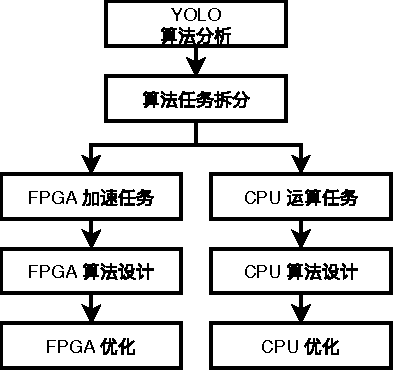
\includegraphics[width=0.40\textwidth]{taskdiv}
    \caption{任务划分流程}
    \label{fig:taskdiv}
\end{figure}

\begin{enumerate}
\item 首先对 CNN 模型进行分析,理解整个算法内部的逻辑以及数据流向。YOLO V2 算法主要有三个步骤:

    \begin{enumerate}
    \item 首先输入任意尺寸的 RGB 格式的图像,将各像素的值归一化到0-1之间,再将图像进行缩放到 $244 \times 244$ 大小,不改变图像的比例,不足处用 0.5 补充,这样就得到了 $244 \times 244 \times 3$ 的矩阵;
    \item 将(1)中得到的矩阵输入 Darknet 网络进行检测,网络检测后输出 $7 \times 7 \times 1024$ 的矩阵;
    \item 对网络输出的结果进行处理,获取输出的边框的信息,再根据各个边框的位置,可信度等,获得最有可能的边框位置。
    \end{enumerate}

\item 在这三个步骤中,步骤(1)的图像预处理和步骤(3)图像的后处理在整个计算中耗时不多,并且计算中设计到了指数运算,这部分如果使用 FPGA 加速需要消耗较多资源,性价比低,因此放在 CPU 上进行计算;
\item YOLO V2 算法中主要有3种类型的层:卷积层、池化层和重排序层。现有的研究表明,卷积层在神经网络的计算中占了大部分计算量,以 Alex-Net 为例,卷积层占了90\% \citep{chen2016eyeriss} 以上的计算量,使用 FPGA 对其并行加速是一种很有效的手段 \citep{farabet2009cnp,peemen2013memory,chen2014diannao}。池化层的运算过程与卷积层类似,不同的是卷积层中使用的是乘加运算而池化层中使用的是比较运算,因此本设计中选择将卷积层和池化层使用 FPGA 进行加速。重排序层的运算过程与内存搬运的过程类似,在 FPGA 中容易实现,因此重排序层也使用 FPGA 进行加速。
\end{enumerate}

\section{基于异构计算的系统体系结构}

考虑到图像的输入及数据存储设备,整个异构系统的结构如图~\ref{fig:system_structure}所示。整个算法运行的流程如下:图像及预训练的权重数据存储在外接的 SD 卡中,PS部分,CPU 通过 SD 卡控制器读取 SD 卡中的图像数据,对其进行预处理后,将其存储到 DDR 内存中;CPU 读取 SD 卡中的权重数据,将其存储在 DDR 内存中。神经网络算法加速器从 DDR 内存中读取预处理过的图像数据及权重数据,对图像进行运算,将运算的输出的结果矩阵存放到 DDR 中。最后 CPU 再从 DDR 中读取神经网络加速器的结果矩阵,进行图像的后处理,将标注完成的图像写回外置的的 SD 卡中。

\begin{figure}[!htbp]
    \centering
    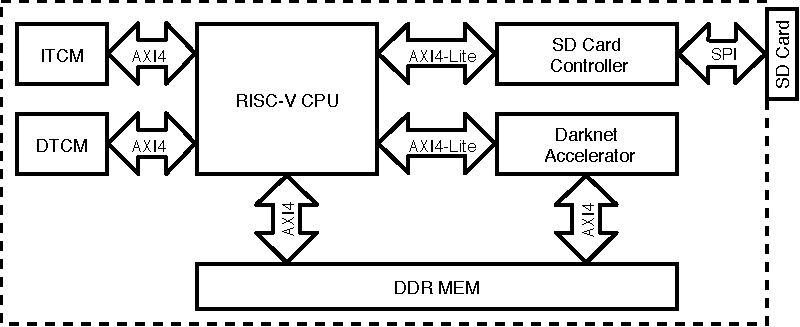
\includegraphics[width=0.70\textwidth]{system_structure}
    \caption{异构系统体系结构}
    \label{fig:system_structure}
\end{figure}

为了保证图像输出的连续性,本设计使用多级缓存,避免让 CPU 读取加速器正在写入的缓存区域。这样输出的实时性得到保证,提高了程序运行的效率。

\section{本章小结}

本章主要介绍了卷积神经网络加速器的总体架构设计,对 YOLO V2 算法进行了任务划分,规划了 SOC 的总体设计。在接下来的第四章和第五章会分别详细介绍 CNN 加速器的设计过程和 SOC 的设计过程。
\chapter{加速器详细设计}\label{chap:accelerator}

本章分两个部分对加速器的设计过程进行说明,第一部分说明了 SIMD 架构的加速器设计的详细过程,第二部分说明了加速器的优化思路及优化过程。

\section{SIMD 架构的卷积神经网络加速器设计}

% 从对 YOLO V2 算法分析中可知,YOLO V2 算法除了路由层之外,其余各层都是将其上一层的输出作为下一层的输入,各层之间串行顺序处理。路由层的任务可以由设置存取地址的偏移实现,CNN 加速器只需要按照算法的流程,从内存对应地址读取数据,在加速器中进行运算,再将结果数据写入内存对应的地址即可。

从对 Darknet 的网络结构分析可知,YOLO V2 算法除了数据输入层之外,各层都是将上一层的输出数据作为本层的输入数据,层间的数据关联性较大,需要串行处理,而层内的数据关联性较小,可以使用 FPGA 进行并行加速。本文设计的加速器运行过程如图~\ref{fig:AcceleratorFlow}所示,CNN 加速器每次从 DDR 内存中读取多块数据写入缓存,CNN 加速器内部的运算单元从缓存获取数据,根据相应的配置参数进行判断,将数据分别交给 CONV、POLL、REORG 模块进行运算,运算的结果数据写入 CNN 加速器的缓存中,最后 CNN 加速器再将计算结果写回 DDR 内存中,由此完成了一整个计算流程。

\begin{figure}[!htbp]
    \centering
    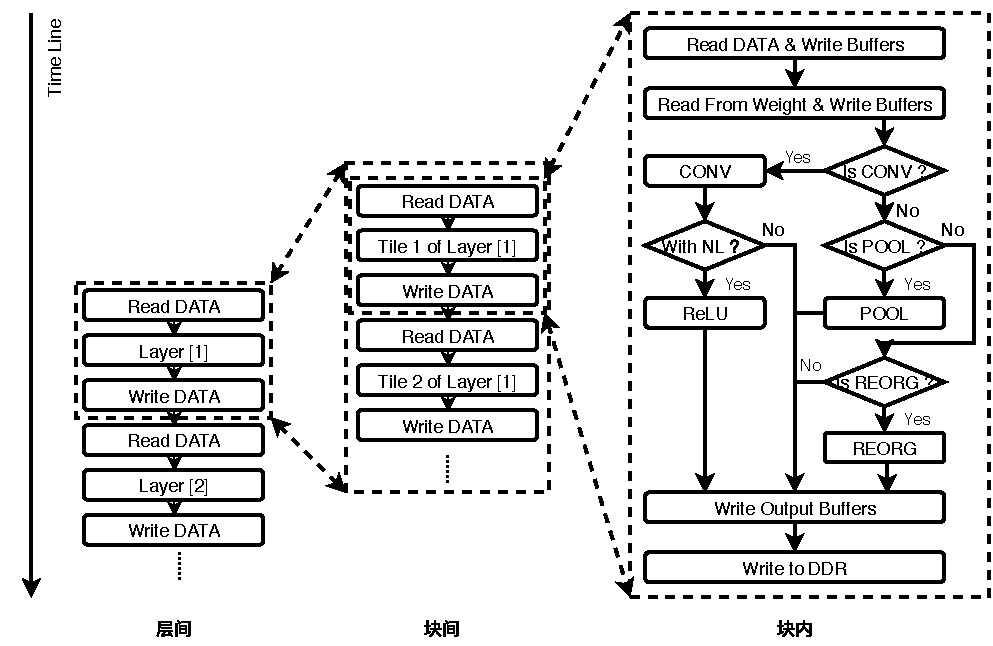
\includegraphics[width=0.9\textwidth]{AcceleratorFlow}
    \caption{CNN 加速器运行流程}
    \label{fig:AcceleratorFlow}
\end{figure}

% 整个加速器运行的流程如图~\ref{fig:AcceleratorFlow}所示,CNN 加速器每次从 DDR 内存中读取多块数据写入缓存,CNN 加速器内部的运算单元从缓存获取数据,根据相应的配置参数进行判断,将数据分别交给 CONV、POLL、REORG 模块进行运算,运算的结果数据写入 CNN 加速器的缓存中,最后 CNN 加速器再将计算结果写回 DDR 内存中,由此完成了一整个计算流程。

CNN 加速器结构如图~\ref{fig:AcceleratorStructure}所示,包含一个 AXI Lite 接口,以及 N 个 AXI Full 接口。其中,AXI Lite 连接在 RISC-V 处理器上,通过此接口,RISC-V 处理器可以对其进行功能的控制,选择 CNN 加速器的计算单元;一个 AXI Full 接口连接在 DDR 内存上,用于获取权重参数;另外的 N-1 个 AXI Full 连接在 DDR 内存上,用来写入或者读取特征图数据。CNN 加速器内部有四个计算单元,分别是 CONV、POLL、REORG 和 ReLU,这四个模块从 CNN 加速器的缓存中获取数据,通过 CNN 加速器中的寄存器控制,分别完成卷积、池化、重排序和激活的计算任务。Data Gather 模块负责生成数据读取地址,并且控制 AXI Full 接口从 DDR 内存中获取数据,将其写入 Input Buffer 模块中进行缓存。Data Scatter 模块负责生成写回地址,并且控制 AXI Full 接口,将 Output Buffer 中的数据写回 DDR 内存中。Weight Buffer 模块缓存负责权重数据。

\begin{figure}[!htbp]
    \centering
    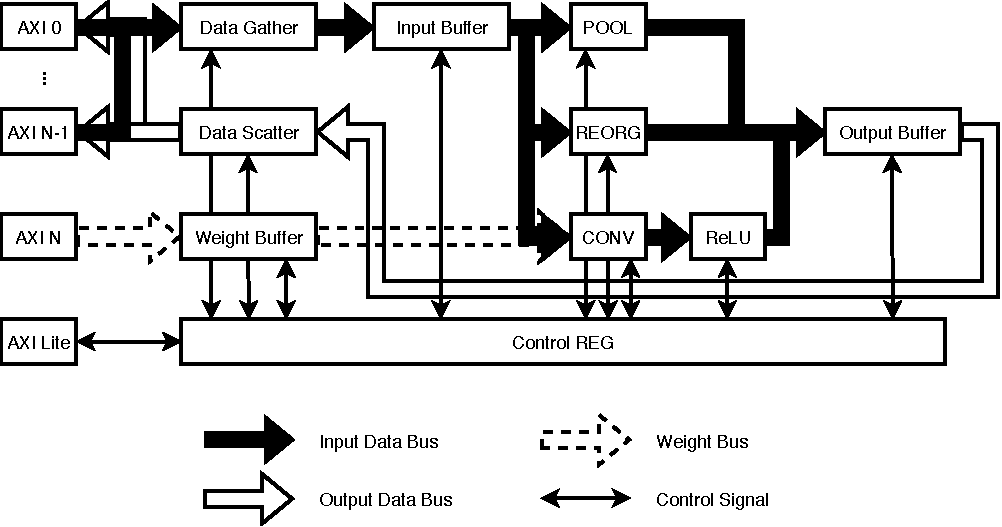
\includegraphics[width=0.9\textwidth]{AcceleratorStructure}
    \caption{CNN 加速器结构}
    \label{fig:AcceleratorStructure}
\end{figure}

负责读写特征图数据的 AXI Full 接口总数量可以由公式~\ref{eq:AxiNum}计算获得:
\begin{equation} \label{eq:AxiNum}
N_{Channel} = Max(N_{in}, N_{out})
\end{equation}

其中 $N_{Channel}$ 表示总的负责读写特征图数据的 AXI Full 接口数量,$N_{in}$ 表示读取特征图需要的 AXI Full 接口的数量,$N_{out}$ 表示输出特征图数据需要的 AXI Full 接口数量。由于 AXI Full 协议是一种全双工的总线协议,所以一条总线上读写操作可以同时进行,互不影响,所以实际上负责读写特征图数据的 AXI Full 接口总数量由读通道和写通道中多的一方决定。

\subsection{数据输入输出模块}

数据输入模块的硬件架构如图~\ref{fig:Input} 所示,Data Scatter 模块从 DDR 内存中获取 $Tif$ 张 $Tix \times Tiy$ 大小的特征图数据,然后依次分发到 CNN 加速器的 $Tif$ 个缓存模块中。数据输出模块的硬件架构如图~\ref{fig:Output} 所示,Data Gather 模块将 CNN 加速器中 $Tof$ 个缓存模块中的数据依次写入到 DDR 内存中。

\begin{figure}[!htbp]
    \centering
    \begin{subfigure}[b]{0.6\textwidth}
        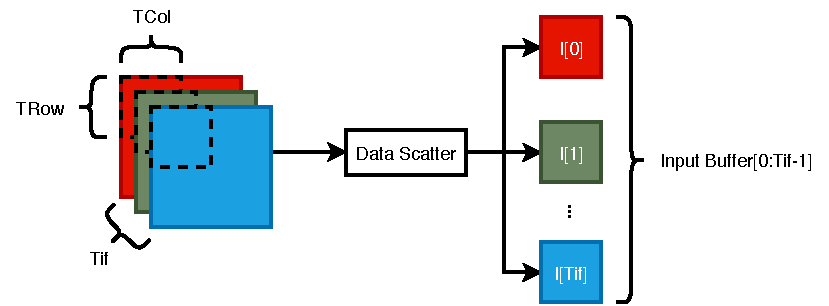
\includegraphics[width=\textwidth]{Input}
        \caption{数据输入模块}
        \label{fig:Input}
    \end{subfigure}
    \\% add desired spacing
    \begin{subfigure}[b]{0.6\textwidth}
        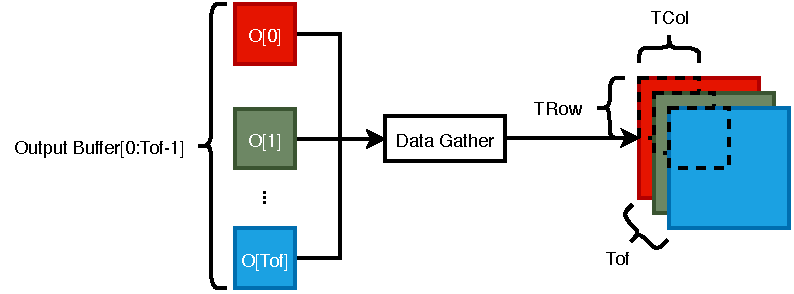
\includegraphics[width=\textwidth]{Output}
        \caption{数据输出模块}
        \label{fig:Output}
    \end{subfigure}
    \caption{数据输入输出模块硬件架构}
\end{figure}

为了保证数据的读写效率,使数据的输入输出部分不至于成为整个加速器的瓶颈,数据输入输出模块中使用双缓存的方案交替读取或者写入数据。

\begin{figure}[!htbp]
    \centering
    \begin{subfigure}[b]{0.6\textwidth}
        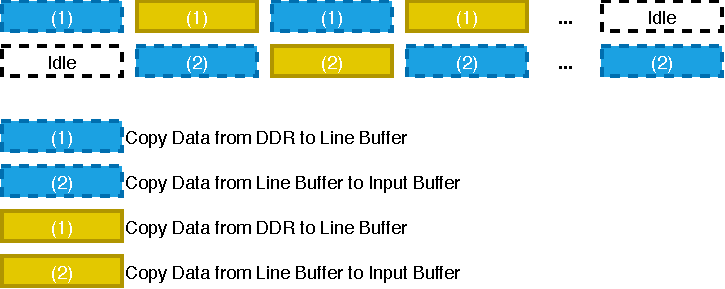
\includegraphics[width=\textwidth]{InputTime}
        \caption{数据输入模块时序}
        \label{fig:InputTime}
    \end{subfigure}
    \\% add desired spacing
    \begin{subfigure}[b]{0.6\textwidth}
        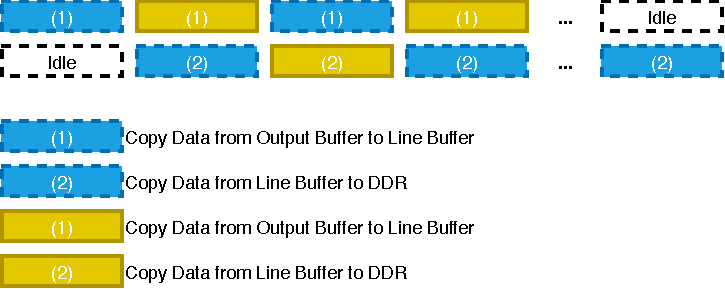
\includegraphics[width=\textwidth]{OutputTime}
        \caption{数据输出模块时序}
        \label{fig:OutputTime}
    \end{subfigure}
    \caption{数据输入输出模块双缓存时序}
\end{figure}

数据输入模块的时序如图~\ref{fig:InputTime} 所示,在流水线中,两个缓存模块交替完成从 DDR 内存中读取数据和将数据分发到 CNN 加速器内部的 Input Buffer 上的任务,考虑到数据读取和数据分发所产生的时延是相同的,因此在理想情况下,使用双缓存模式后,数据输入模块产生的时延仅为原先单缓存模式下的 $\frac{1}{2}$。

数据输出模块的时序如图~\ref{fig:OutputTime} 所示,在流水线中,两个缓存模块交替完成从 CNN 加速器内的 Output Buffer 上获取数据和将数据写入 DDR 内存的任务。和数据输入模块的时序相似,在理想情况下,使用双缓存模式后,数据输出模块产生的时延仅为原先单缓存模式下的 $\frac{1}{2}$。

\subsection{CONV 卷积模块}

由于卷积层有大量的乘加运算,占据了整个 CNN 计算的大部分时间,因此在硬件加速中,本设计将卷积层进行不同维度的展开,通过设计相应的并行乘加运算单元,来达到加速卷积计算的效果。基本的维度展开主要分以下 4 种:

\subsubsection{卷积核维度的展开}

\begin{figure}[!htbp]
    \centering
    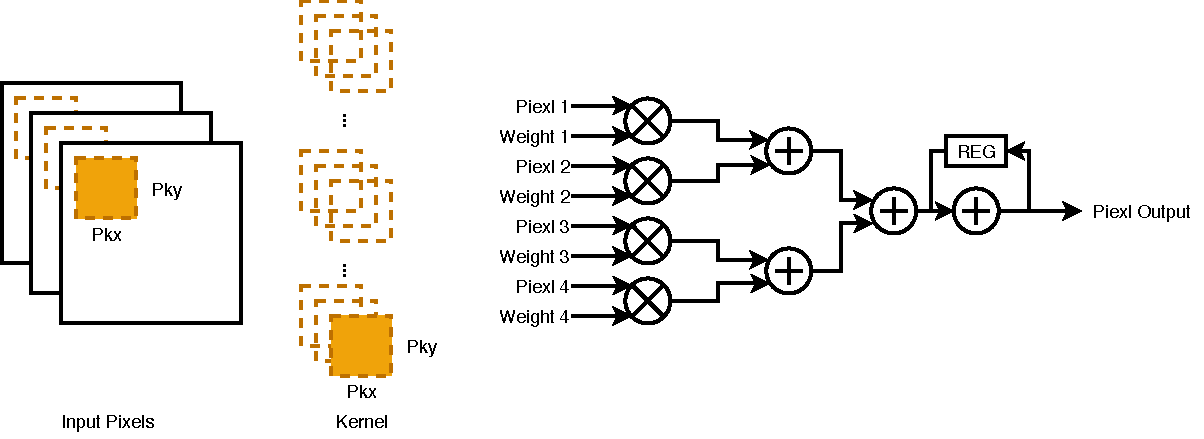
\includegraphics[width=0.8\textwidth]{UnfoldKernel}
    \caption{卷积核维度展开硬件架构}
    \label{fig:UnfoldKernel}
\end{figure}

如图~\ref{fig:UnfoldKernel}所示,展开卷积核的宽度 $Pkx$ 和卷积核的高度 $Pky$。在每个时钟周期里,同一输入特征图的相邻的 $Pkx \times Pky$ 个相邻的像素与卷积核对应位置的权重数据进行并行的乘法运算,乘法运算的结果通过一个深度为 $log_2{Pkx \times Pky}$ 的加法树相加得到中间结果,累加的结果存放在一个寄存器中。该维度展开卷积运算,消耗的资源为 $Pkx \times Pky$ 个乘法器、一个深度为 $log_2{Pkx \times Pky}$ 的加法树和一个累加器。

\subsubsection{输入特征图数维度的展开}

\begin{figure}[!htbp]
    \centering
    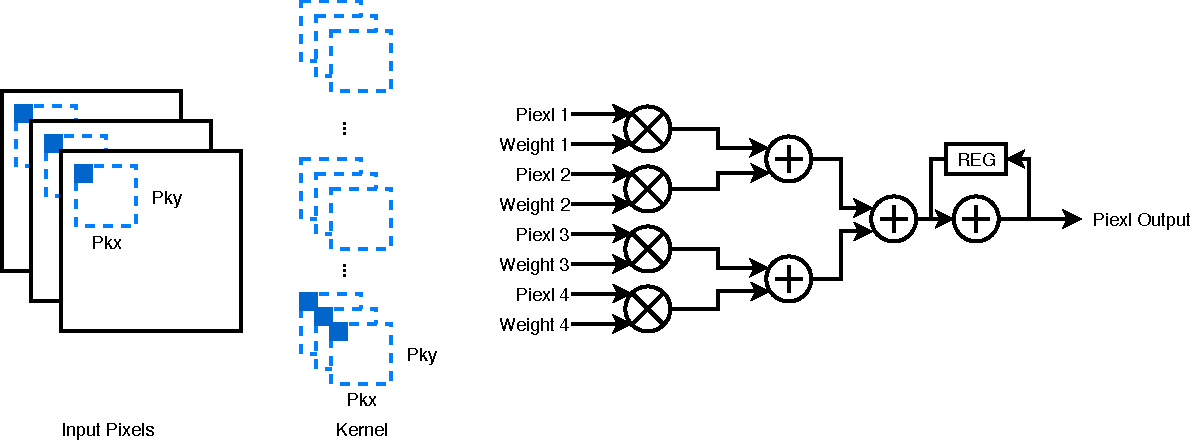
\includegraphics[width=0.8\textwidth]{UnfoldInput}
    \caption{输入特征图数维度展开硬件架构}
    \label{fig:UnfoldInput}
\end{figure}

如图~\ref{fig:UnfoldInput}所示,展开 $Pif$ 个输入特征图。在每个时钟周期里,同时从 $Pif$ 个输入特征图的同一位置读取一个像素与卷积核对应位置的权重数据进行乘法运算,乘法运算的结果通过一个深度为 $log_2{Pif}$ 的加法树相加得到中间结果,累加的结果存放在一个寄存器中。该维度展开卷积运算,消耗的资源为 $Pif$ 个乘法器、一个深度为 $log_2{Pif}$ 的加法树和一个累加器。

\subsubsection{输出特征图维度的展开}

\begin{figure}[!htbp]
    \centering
    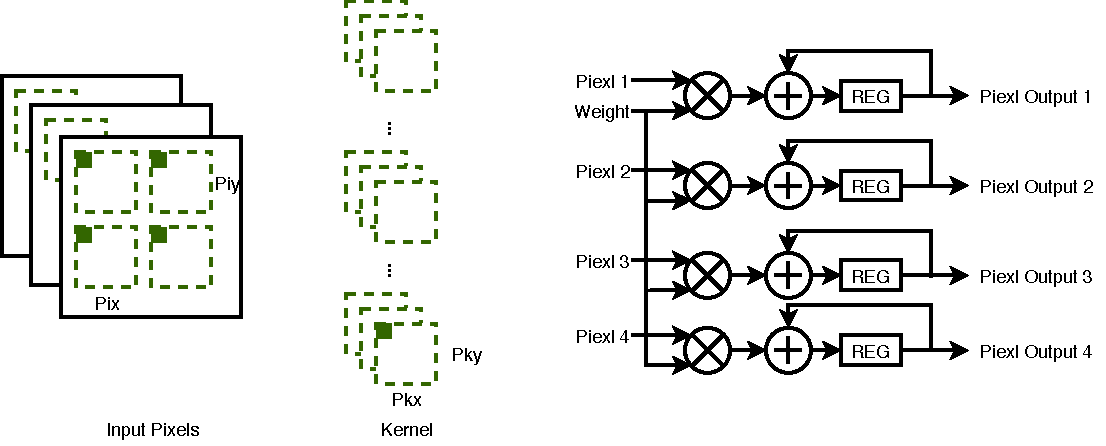
\includegraphics[width=0.8\textwidth]{UnfoldOutput}
    \caption{输出特征图维度展开硬件架构}
    \label{fig:UnfoldOutput}
\end{figure}

如图~\ref{fig:UnfoldOutput}所示,展开输出特征图的宽度 $Pix$ 和卷积核的高度 $Piy$。在每个时钟周期里,计算同一输出特征图的相邻的 $Pix \times Piy$ 个相邻的像素的值。该过程与卷积核维度的展开的运算类似。

\subsubsection{输出特征图数维度的展开}

\begin{figure}[!htbp]
    \centering
    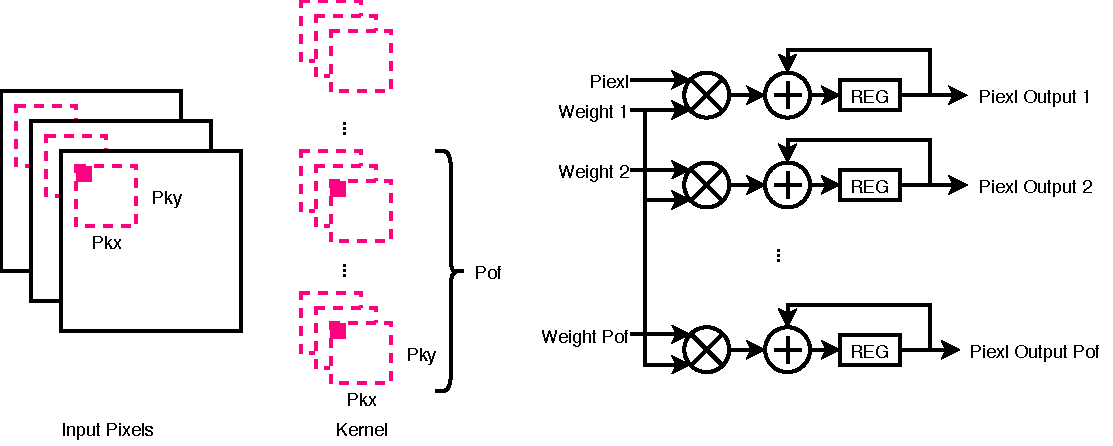
\includegraphics[width=0.8\textwidth]{UnfoldOutputNum}
    \caption{输出特征图数维度展开硬件架构}
    \label{fig:UnfoldOutputNum}
\end{figure}

如图~\ref{fig:UnfoldOutputNum}所示,展开 $Pof$ 个输出特征图。在每个时钟周期里,同时将同一个输入特征图的一个像素与 $Pof$ 个卷积核对应位置的权重数据进行乘法运算,乘法运算的结果通过一个深度为 $log_2{Pof}$ 的加法树相加得到中间结果,累加的结果存放在一个寄存器中。该维度展开卷积运算,消耗的资源为 $Pof$ 个乘法器、一个深度为 $log_2{Pof}$ 的加法树和一个累加器。

\subsubsection{卷积展开设计}

由于在 FPGA 中,图像数据是以数据流的形式进行传输的,即在流水线中,每个时钟周期传输一个像素的数据,如果想一个时钟周期同时访问 $N$ 个像素的数据,就需要 $N$ 条数据总线。但由于在本设计中,特征图数据是存储在外置的 DDR 中的,同时访问 $N$ 个像素的数据违背了 DDR 的工作原理,因此任然需要排队等待。所以这种需要同时访问多个像素数据的优化方式在访存部分会形成瓶颈,无法达到有效的加速效果。而展开方法(1)卷积核维度的展开与展开方法(3)输出特征图维度的展开正是有这种多个像素同时读取的需求,因此在本设计中使用的卷积展开方法主要是展开方法(2)输入特征图数维度的展开与展开方法(4)输出特征图数维度展开的结合使用。

\begin{figure}[!htbp]
    \centering
    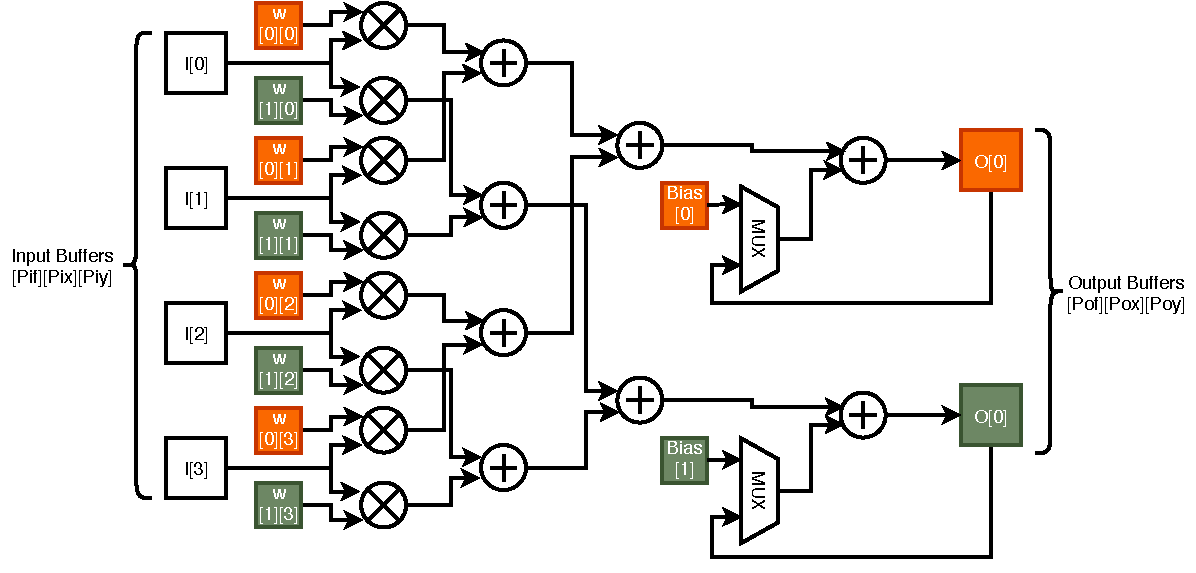
\includegraphics[width=0.8\textwidth]{Unfold}
    \caption{卷积模块硬件架构}
    \label{fig:Unfold}
\end{figure}

如图~\ref{fig:Unfold}所示,通过对输入特征图数维度于输出特征图数维度进行二维展开。以输入特征图数 $Pif = 4$ 和输出特征图数 $Pof = 2$ 为例,展开度为 $Pif \times Pof = 8$。在一个时钟周期内,同时从 $Pif$ 个输入特征图的同一位置读取一个像素分别和 $Pof$ 个卷积核对应的权重数据相乘,再将乘法的结果通过一个深度为 $log_2{Pif\times Pof}$ 的加法树相加,加法树输出的结果在通过一个累加器将局部运算的结果进行累加,最终的结果存放在 CNN 加速器的寄存器中。该展开方式消耗 $Pif \times Pof$ 个乘法器,一个深度为 $log_2{Pif \times Pof}$ 的加法树和一个累加器。

在内存访问速度不是瓶颈的情况下,即每个时钟周期可以获得一个输入特征图的像素,该展开方式进行卷积计算产生的时延如公式~\ref{eq:convlatency}所示。式中 $Latency_{CONV}$ 为一层卷积计算的总时延;$Const_{CONV}$ 为一个常量,代表了数据充满流水线所需要的时间;$Nky$ 与 $Nkx$ 分别表示输入特征图的高度和宽度;$Toy$ 和 $Tox$ 表示卷积核的高度和宽度。 
\begin{equation} \label{eq:convlatency}
Latency_{CONV} = (Const_{CONV} + Nky \times Nkx \times Toy \times Tox)/Freq
\end{equation}

可以看到,在该展开方式下,卷积运算的总时延与单层输入特征图,单层输出特征图的时延相当。因此在该展开方式下,卷积计算的总时延仅为原本的 $\frac{1}{Pof \times Pif}$,因此该展开方式可以有效的对卷积运算进行加速。

\subsection{POOL 池化模块}

由于图像中相邻位置的像素有着相似的值,卷积层的输出特征图同样也会在相邻区域有值相似的像素,因此去除这些相似值的像素并不会使特征图损失很多信息,并且通过去除这些相似的像素可以极大的减少参数数量,从而降低后续卷积运算的计算量,池化层就是完成了这个任务。池化运算与卷积运算类似,YOLO V2 算法中所有的池化层都是大小为 $2 \times 2$,步长 $S = 2$ 的最大池化。因此池化加速模块的设计可以参考卷积模块的设计,不同的是池化模块只需要对单一的输入特征图进行运算,并且运算单元由原先卷积模块中的乘加运算单元换成了比较运算单元。

\begin{figure}[!htbp]
    \centering
    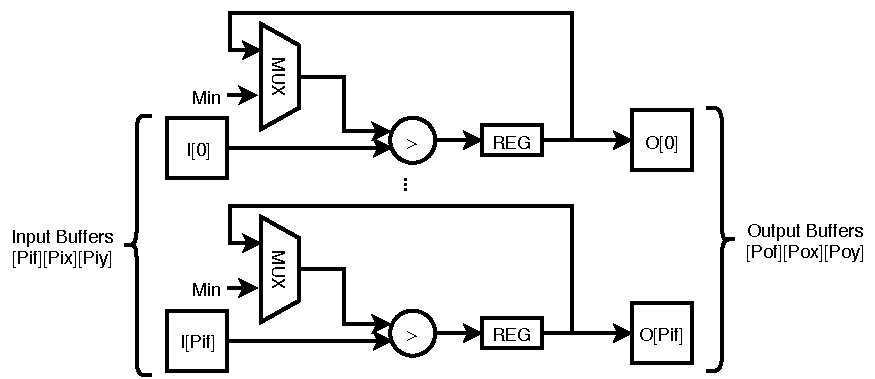
\includegraphics[width=0.80\textwidth]{pool}
    \caption{池化模块硬件架构}
    \label{fig:pool}
\end{figure}

如图~\ref{fig:pool} 所示,池化模块在运算过程中,同时从 $Pif$ 个输入特征图的同一位置获取一个像素,并与当前的最大值进行比较,在比较完成后,将得到的最大值写入输出缓存中。该结构的池化模块消耗 $Pif$ 个比较器和 $Pif$ 个寄存器。该池化运算加速模块的计算时延如公式~\ref{eq:pool}所示:
\begin{equation} \label{eq:pool}
Latency_{POOL} = (Const_{POOL} + Nky \times Nkx \times Toy \times Tox)/Freq
\end{equation}

式中 $Latency_{POOL}$ 为一层池化计算的总时延;$Const_{POOL}$ 为一个常量,代表了数据充满流水线所需要的时间;$Nky$ 与 $Nkx$ 分别表示输入特征图的高度和宽度;$Toy$ 和 $Tox$ 表示池化核的高度和宽度。 

\subsection{REORG 重排序模块}

重排序层的作用主要是对输入特征图进行一个拆分,将输入特征图相邻位置的像素分别输出到不同的特征图上。该过程的运算与池化模块的运算过程相似,不同的是池化模块将一个输入特征图输出到一个输出特征图,而重排序模块是将一个输入特征图输出到多个输出特征图。重排序模块的硬件架构如图~\ref{fig:reorg}所示。

\begin{figure}[!htbp]
    \centering
    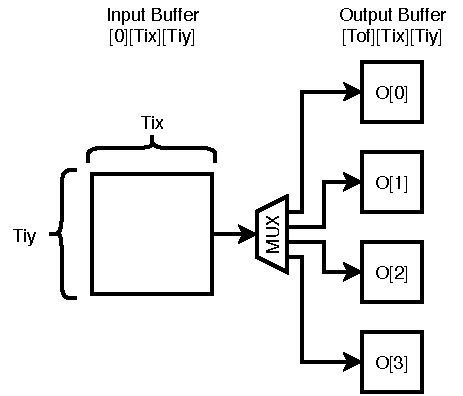
\includegraphics[width=0.40\textwidth]{reorg}
    \caption{重排序模块硬件架构}
    \label{fig:reorg}
\end{figure}

由于 YOLO V2 中的重排序层是 $Nky=Nkx=S=2$ 的结构,因此重排序层需要1个输入缓存模块和4个输出缓存模块,重排序模块的计算时延如公式~\ref{eq:reorg}所示:
\begin{equation} \label{eq:reorg}
Latency_{REORG} = (Const_{REORG} + Nky \times Nkx)/Freq
\end{equation}

式中 $Latency_{REORG}$ 为一层重排序计算的总时延;$Const_{REORG}$ 为一个常量,代表了数据充满流水线所需要的时间;$Nky$ 与 $Nkx$ 分别表示输入特征图的高度和宽度。

\section{CNN 加速器优化}

\subsection{乒乓缓冲优化}

乒乓缓冲在 FPGA 设计中是一种典型的以面积换时间的做法,在本次设计的 CNN 加速器中,我们在 CNN 加速器的数据输入端口和数据输出端口使用了乒乓缓冲的结构进行优化。因此该 CNN 加速器在流水线模式下运行时可以使数据传输产生的时延与数据运算产生的时延相重叠,加速器运算的总时延的计算如公式~\ref{eq:latency}所示:
\begin{equation} \label{eq:latency}
Latency_{ALL} = Max(Latency_{load},Latency_{compute},Latency_{store})
\end{equation}

式中 $Latency_{ALL}$、$Latency_{load}$、$Latency_{compute}$、$Latency_{store}$ 分别代表 CNN 加速器运算的总时延、从 DDR 内存中读取数据所产生的时延、加速器计算所产生的时延、将数据写回 DDR 内存中的所产生的时延。

\subsection{多数据通道传输优化}

由于 DDR 内存的带宽远大于一条 AXI4 总线的带宽,为了充分利用 DDR 内存的带宽,减少数据传输过程中产生的时延,在本设计中使用了多数据通道传输的优化方式。

\begin{figure}[!htbp]
    \centering
    \begin{subfigure}[b]{0.70\textwidth}
        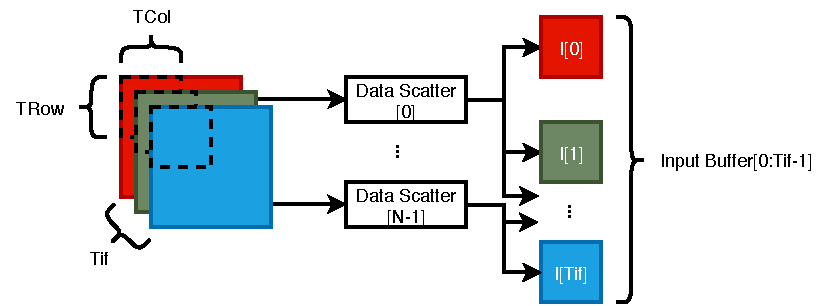
\includegraphics[width=\textwidth]{InputMult}
        \caption{数据输入模块}
        \label{fig:InputMult}
    \end{subfigure}
    \\% add desired spacing
    \begin{subfigure}[b]{0.70\textwidth}
        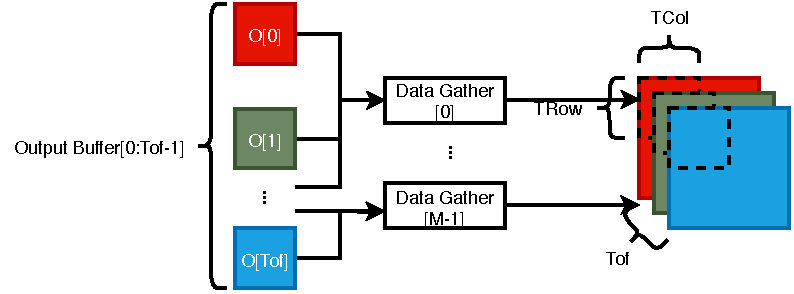
\includegraphics[width=\textwidth]{OutputMult}
        \caption{数据输出模块}
        \label{fig:OutputMult}
    \end{subfigure}
    \caption{多数据通道传输优化硬件架构}
\end{figure}

数据输入模块的多数据通道传输优化硬件架构如图~\ref{fig:InputMult} 所示,模块内部有多个独立的 Data Scatter 模块,每个模块有一条独立的 AXI4 总线,每个 Data Scatter 模块负责一部分数据缓存模块,因此多个 Data Scatter 模块可以并行地从 DDR 内存中读取特征图数据,并将数据分发到其负责的缓存模块上,从而提高了 DDR 内存的带宽利用率。

数据输出模块的多数据通道传输优化硬件架构如图~\ref{fig:OutputMult} 所示,与数据输入模块的优化思路相似,在模块内部使用多个独立的 Data Gather 模块,每个模块有一条独立的 AXI4 总线,因此多个 Data Gather 模块可以并行的将其负责的一部分缓存模块中的数据写入到 DDR 内存中 。

\section{本章小结}

本章对 CNN 加速器进行了详细的设计及优化。具体说明了四种卷积循环的展开模式以及各模式产生的时延和局限性,最终选取了输入特征图数维度的展开和输出特征图数维度的展开相结合的模式,从而在硬件资源的允许范围内,尽可能多的减少卷积运算产生的时延。同时由于硬件资源的限制,无法将 YOLO V2 模型的所有层同时进行硬件加速,因此采取了每次加速一层中一部分的做法,该方法类似于 FPGA 中状态机的思路,是一种用时间换面积的做法。由于该方法涉及大量的内存读写,为了使内存读写的时延不成为 CNN 加速器的瓶颈,加速器内部使用了双缓存和多数据通道的优化方法,保证了在流水线运行模式下,内存的读写时间可以被卷积运算的时间所掩盖,从而尽量减少内存的读写所产生的时延对加速器性能造成的影响。
\chapter{RISC-V \ SOC设计}\label{chap:soc}

由于神经网络中的卷积计算、池化计算及全连接计算等都在加速器中完成,而网络中的图像预处理、softmax层计算等耗时较短的操作则由 RISC-V 处理器来完成。为了让 CNN 加速器和 RISC-V 处理器协同工作,在本章中我们设计了一个通用的 SOC,将 CNN 加速器作为 RISC-V 处理器的一个外设,由 RSIC-V 处理器进行流程控制和图像预处理、softmax层计算等工作,CNN 加速器负责主要的卷积神经网络计算任务。为了提高设计效率,本设计中将 RISC-V 处理器和神经网络加速器封装成带有 AXI4 总线接口 的 IP,通过 AXI4 总线与 UART、GPIO、定时器等外设连接。下面详细介绍 SOC 的设计过程。

\section{SOC 整体设计}

由于目前 RISC-V 基金会还没有发布标准的 RISC-V 调试架构文档\citep{胡振波2018手把手教你设计},因此目前开源的几款 RISC-V 处理器大多不带调试机制,这就给软件调试带来了不便之处,为此这里参考了 PYNQ MicroBlaze Subsystem 的设计 \citep{PYNQ_MB},在 ZYNQ 芯片上运行 Linux 系统与 RISC-V 处理器共享内存来完成程序的下载过程。

\begin{figure}[!htbp]
    \centering
    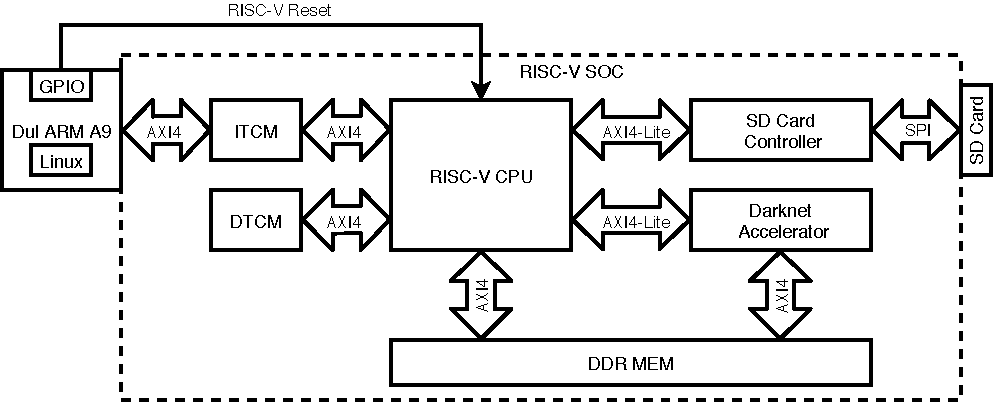
\includegraphics[width=0.80\textwidth]{soc}
    \caption{RISC-V SOC 架构}
    \label{fig:soc}
\end{figure}

SOC 整体的结构设计如图~\ref{fig:soc}所示。在本设计中,将 SOC 部分在 ZYNQ 的 PL 部分实现。RISC-V 的 ITCM 使用一个双端口 Block RAM 实现,ITCM 的一个端口与 RISC-V 处理器连接,其另一个端口通过 AXI4 总线与 ZYNQ 上的 ARM 核相连,ARM 核可以读写这块 ITCM 中的数据。在 ZYNQ 的 双核 ARM A9 上运行 linux 系统,在该系统上使用交叉编译工具编译 RISC-V 的软件程序,将编译后的二进制文件放入 RISC-V 处理器的 ITCM 中,再复位 RISC-V 处理器,便可以使 RISC-V 处理器执行相应的程序。

% \section{RISC-V 处理器选择}

% \# 需要各 RISC-V 处理器的性能数据对比。

\section{SOC 硬件详细设计}

本 SOC 主要包含 RISC-V 处理器,集成 ROM、RAM,包含了基本的外设(包括GPIO、UART等)以及神经网络加速器,各模块之间通过 AXI4 总线连接。

\subsection{RISC-V处理器接口描述}
Ibex处理器的结构如图~\ref{fig:blockdigram}所示,Ibex处理器的接口主要包含6个部分:

\begin{figure}[htbp]
    \centering
    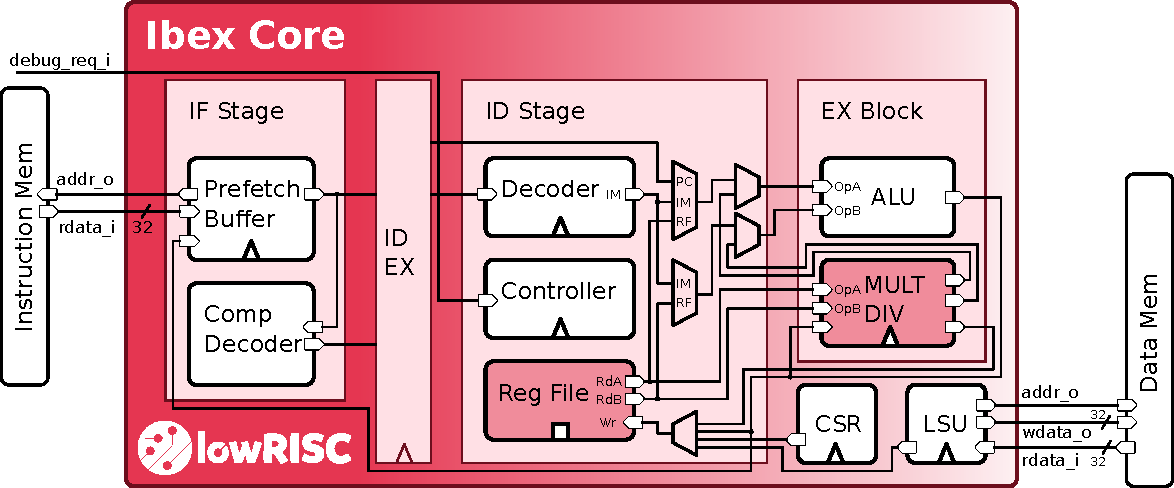
\includegraphics[width=0.9\textwidth]{blockdigram}
    \caption{Ibex处理器结构}
    \label{fig:blockdigram}
\end{figure}

\begin{enumerate}
    \item 时钟和复位接口;
    \item 控制接口;
    \item 指令私有总线接口;
    \item 数据私有总线接口;
    \item 中断接口;
    \item Debug接口。
\end{enumerate}

%\subsection{私有总线转AHB总线}
%由于Ibex使用的是私有总线,而本SOC平台的为了保证通用性,使用的是AMBA总线,因此需要将Ibex私用总线转换为AMBA总线。
%Ibex私有总线时序如图\ref{fig:ibexsx}所示:
%
%\begin{figure}[htbp]
%   \centering
%   \includegraphics[width=\textwidth]{ibex私有总线时序}
%   \caption{Ibex私有总线时序}
%   \label{fig:ibexsx}
%\end{figure}
%
%AHB总线的时序如图\ref{fig:ahbsx}所示:
%
%\begin{figure}[htbp]
%   \centering
%   \includegraphics[width=\textwidth]{AHB总线时序}
%   \caption{AHB总线时序}
%   \label{fig:ahbsx}
%\end{figure}

\subsection{SOC片上存储资源}
本SOC中的片上存储器资源分为ITCM和DTCM,其结构如图~\ref{fig:sram} 所示。其中 ITCM(Instruction Tightly Coupled Memory)为 RISC-V 处理器内核私有的指令寄存器,其大小可以配置,默认设置为 64Kb;默认的起始地址是 0x8000\_0000;由于 ITCM 是用来存放指令的,所以 RISC-V 处理器在正常运行时,这块区域是只读的,为了实现程序的掉电保存,需要将程序存放在外置的非易失性存储器上,在处理器复位后,使用 Load 和 Store 指令将程序搬运到 ITCM 中,这个阶段 ITCM 为可读写状态。因此 ITCM 使用一个双端口 Block RAM 实现,其有两个读写接口,一个读写接口直连处理器的指令总线接口,另一个接口通过一个仲裁器分别连接了处理器的数据总线接口和Debug模块的数据接口。

DTCM(Data Tightly Coupled Memory)为 RISC-V 处理器内核私有的数据存储器,其大小可以配置,默认为 64Kb;默认的起始地址是 0x9000\_0000;DTCM 用来存放程序运行中的数据,相当于处理器的内存,因此在通常状态下,DTCM 都是可读写的,所以 DTCM 使用一个单端口 RAM 实现,其接口直接连接在处理器的数据总线接口上。

\begin{figure}[htbp]
    \centering
    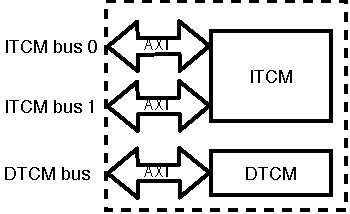
\includegraphics[width=0.4\textwidth]{sram}
    \caption{片上存储器资源结构框图}
    \label{fig:sram}
\end{figure}

% \begin{enumerate}
%     \item 大小可配置,默认设置为64Kb;
%     \item 可配置地址区间,默认起始地址为0x8000\_0000;
%     \item ITCM虽然主要用来存放指令,但是其地址区间也可以被处理器核的Load和Store指令访问,从而实现将存储在片外存储器上的指令加载到片内ITCM上,实现程序的掉电保存。
% \end{enumerate}

% DTCM为RISC-V处理器内核私有的数据存储器,其特性如下:
% \begin{enumerate}
%     \item 大小可配置,默认设置为64Kb;
%     \item 可配置地址区间,默认起始地址为0x9000\_0000;
%     \item DTCM只能被处理器的数据存储器访问指令访问,因此只能用来存放数据。
% \end{enumerate}

% ITCM使用一个双端口RAM实现,其有两个读写接口,一个读写接口直连处理器的指令总线接口,另一个接口通过一个仲裁器分别连接了处理器的数据总线接口和Debug模块的数据接口。

% DTCM使用一个单端口RAM实现,其接口直接连接在处理器的数据总线接口上。

\subsection{SOC外设资源}
\begin{enumerate}
    \item UART 

    本SOC中实现了一个URAT外设,采用 AXI Lite 总线接口,结构如图~\ref{fig:uart} 所示。该 UART 在接收端使用 16 倍波特率的采样频率进行采样;数据格式为 8 位数据,没有奇偶校验位,1 位起始位,1 位停止位;波特率由内部寄存器控制,支持软件调节;支持全双工的接收和发送数据,内部带有接收缓存和发送缓存;中断产生的阈值由内部寄存器控制,支持软件调节。
    
    \begin{figure}[htbp]
        \centering
        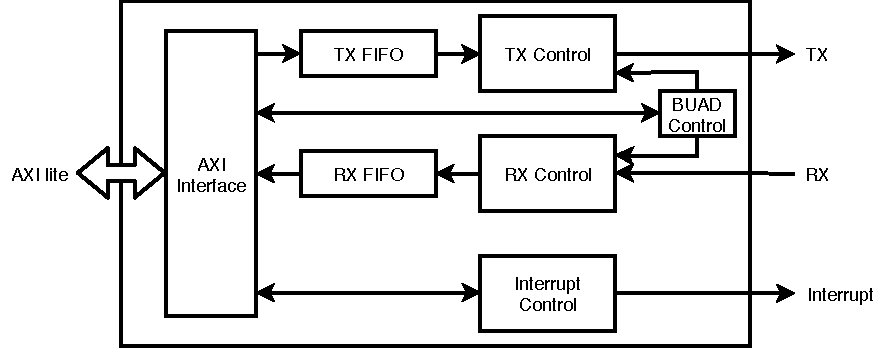
\includegraphics[width=0.7\textwidth]{uart}
        \caption{UART结构框图}
        \label{fig:uart}
    \end{figure}
    
    % \begin{itemize}
    %     \item 支持发送和接收数据能力;
    %     \item 支持8-N-1数据传输格式:即8位数据位、没有奇偶校验位、1位起始位、1位停止位;
    %     \item 支持软件可编程的阈值产生中断;
    %     \item 支持软件可编程的波特率调节;
    %     \item 在接收端采用16倍波特率的采样频率进行采样接收数据。
    % \end{itemize}
    
    \item GPIO
    
    本SOC中实现了一个双通道 32 位GPIO,采用 AXI Lite 总线接口,其结构如图~\ref{fig:gpio} 所示。每个通道有 32 位的双向 I/O 口,每位 I/O 口的方向由内部寄存器控制,支持软件调节;内部带有一个中断控制器,在 I/O 口为输入时,可以产生中断信号。
    
    \begin{figure}[htbp]
        \centering
        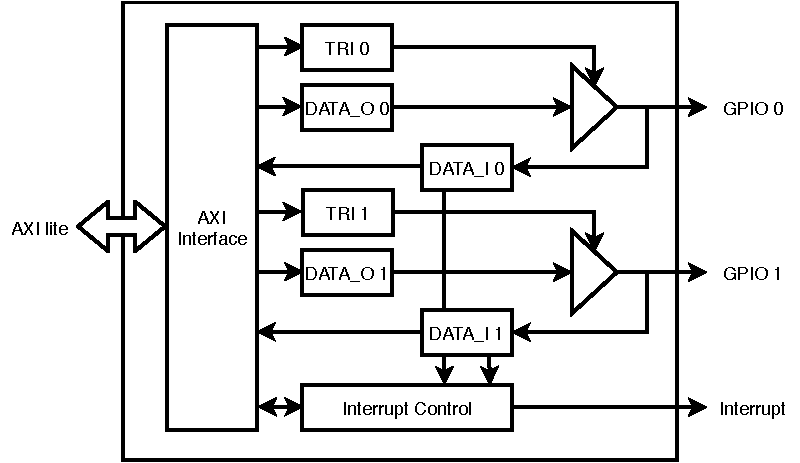
\includegraphics[width=0.7\textwidth]{gpio}
        \caption{GPIO结构框图}
        \label{fig:gpio}
    \end{figure}
    
    % \begin{itemize}
    %     \item 每个GPIO控制器提供一组32个I/O的通用输入输出接口;
    %     \item 每个I/O均可直接接受软件编程的可配置寄存器控制,此时I/O的表现为输出;
    %     \item 每个I/O均可直接接受硬件接口控制信号,此时I/O表现为输入;
    %     \item 每个I/O均可产生中断。
    % \end{itemize}
    
    \item RTC
    
    RTC(Real-Time Clock)是MCU中常用的模块,用于给程序运行提供精确计时的功能。本 SOC 中设计了一个 RTC 模块,其结构如图~\ref{fig:rtc} 所示。本设计中的 RTC 包含了两个独立的 32 位计数器,其触发信号为 CPU 的时钟,这两个计数器可以在其内部寄存器的控制下级联成一个 64 位的计数器。计数器的初始值可由内部寄存器控制,计数器向上计数,加满之后再加一,就会产生溢出,从而通知中断控制器产生中断。
    
    \begin{figure}[htbp]
        \centering
        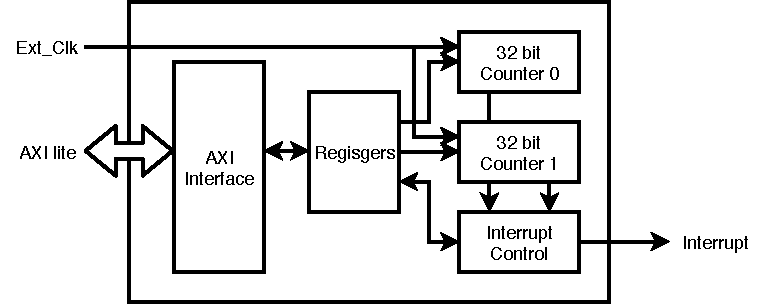
\includegraphics[width=0.7\textwidth]{rtc}
        \caption{RTC结构框图}
        \label{fig:rtc}
    \end{figure}
    
    % \begin{itemize}
    %     \item RTC本质上是两个独立的32位计数器,计数器在被使能后每个周期自增加一;
    %     \item 两个独立的RTC受软件编程控制可级联为一个64位计数器;
    %     \item 支持可编程寄存器设定计数器的比较阈值,一旦RTC计数器的比较值达到阈值,可以产生中断。
    % \end{itemize}
    
\end{enumerate}

\section{本章小结}

本章详细介绍了 SOC 的设计过程,采用了一种以 ZYNQ 架构为基础的通用 RISC-V SOC 设计,方便对于没有调试接口的 RISC-V 处理器进行程序调试和程序下载运行的操作,同时介绍了部分外设的设计过程。


% \chapter{PS部分设计}\label{chap:ps}

\section{研究背景及意义}

\section{国内外研究现状}

\section{研究内容及结构安排}
\chapter{测试与分析}\label{chap:test}

\section{CNN 加速器测试实验环境}

本设计中使用的 CNN 模型是 YOLO V2 Tiny\citep{redmon2017yolo9000};数据集为 VOC 2007 数据集\citep{everingham2007pascal},该数据集包含了 20 个类;FPGA 平台为 PYNQ-Z2 开发板(Dual ARM A9 + FPGA)。

硬件设计工具使用如下:CNN 加速器使用 Vivado HLS 2018.2 工具设计,硬件工程使用 Vivado 2018.2 工具设计;软件设计工具如下:使用 riscv32-unknown-elf-gcc 交叉编译工具对 RISC-V 处理器的程序进行编译。

\section{对比测试环境}

为了直观了解 CNN 加速器的加速效果,设计了3组对照实验进行对比分析,分别如下:

X86架构 CPU 平台:CPU为 Intel i7-9700K,8核心,频率为 4.9 GHz;32GB 运行内存;

嵌入式 CPU 平台:树莓派 3B,CPU 为四核 ARM Cortex-A53,频率为 1.2 GHz;1 GB 的运行内存;

嵌入式 GPU 平台:NVIDIA Jetson Nano,四核 ARM Cortex-A57 MPCore 处理器,频率为 1.43GHz;GPU 为 Maxwell 架构,配备 128 个 CUDA 核心;4GB 运行内存。

\section{CNN 加速器资源消耗评估}

% PYNQ-Z2 开发板上使用的 ZYNQ 7020 芯片有 220 个 DSP 单元,在当前的 CNN 加速器的设计中,卷积过程使用定点 16 位精度的乘法运算,因此每个乘法器会消耗一个 DSP 单元,加法器消耗 LUT,不消耗 DSP。CNN 加速器的运行频率为 150 MHz,因此可以计算出本系统的性能上限为 66GOPS($220 \times 150 \times 2 / 1000 = 66$)。

% PYNQ-Z2 开发板上的内存型号为 32bit DDR3-1066,理论最大带宽为 4.26 GB/s;由 UG585 \citep{xilinx2015zynq} 可知,实际上带宽利用率为总带宽的 75 \% 左右,所以本系统的最大带宽为 3.198 GB/s。根据文献 \citep{陈辰2019基于}中的计算可知,在兼顾性能与功耗的情况下,选取设计参数为:$Tif=2,Tof=86,Toy=26,Tox=36$,在使用该参数的情况下,CNN 加速器的算力为 30.33 GOPS。

整个异构运算系统的设计连接如图~\ref{fig:VivadoStructure}所示,其中 YOLOV2\_FPGA 为基于 YOLO V2 算法的设计 CNN 加速器 IP 核。RISCV\_Processor 为 RISC-V 处理器 IP 核。其余部分是 SOC 中的一些基本外设。YOLO V2 算法加速器有 1 个 AXI-Lite Slave 接口,连接在 RISC-V 处理器的数据总线接口上,负责状态寄存器的控制;还有 5 个 AXI Master 接口分别与 DDR 的 HP[0:3] 接口连接,其中有两个 AXI Master 接口连接在 HP[3] 上。CNN 加速器及其数据通路运行在 150 MHz 的时钟频率下,SOC 中其他部分运行在 100 MHz 的时钟频率下。

\begin{figure}[!htbp]
    \centering
    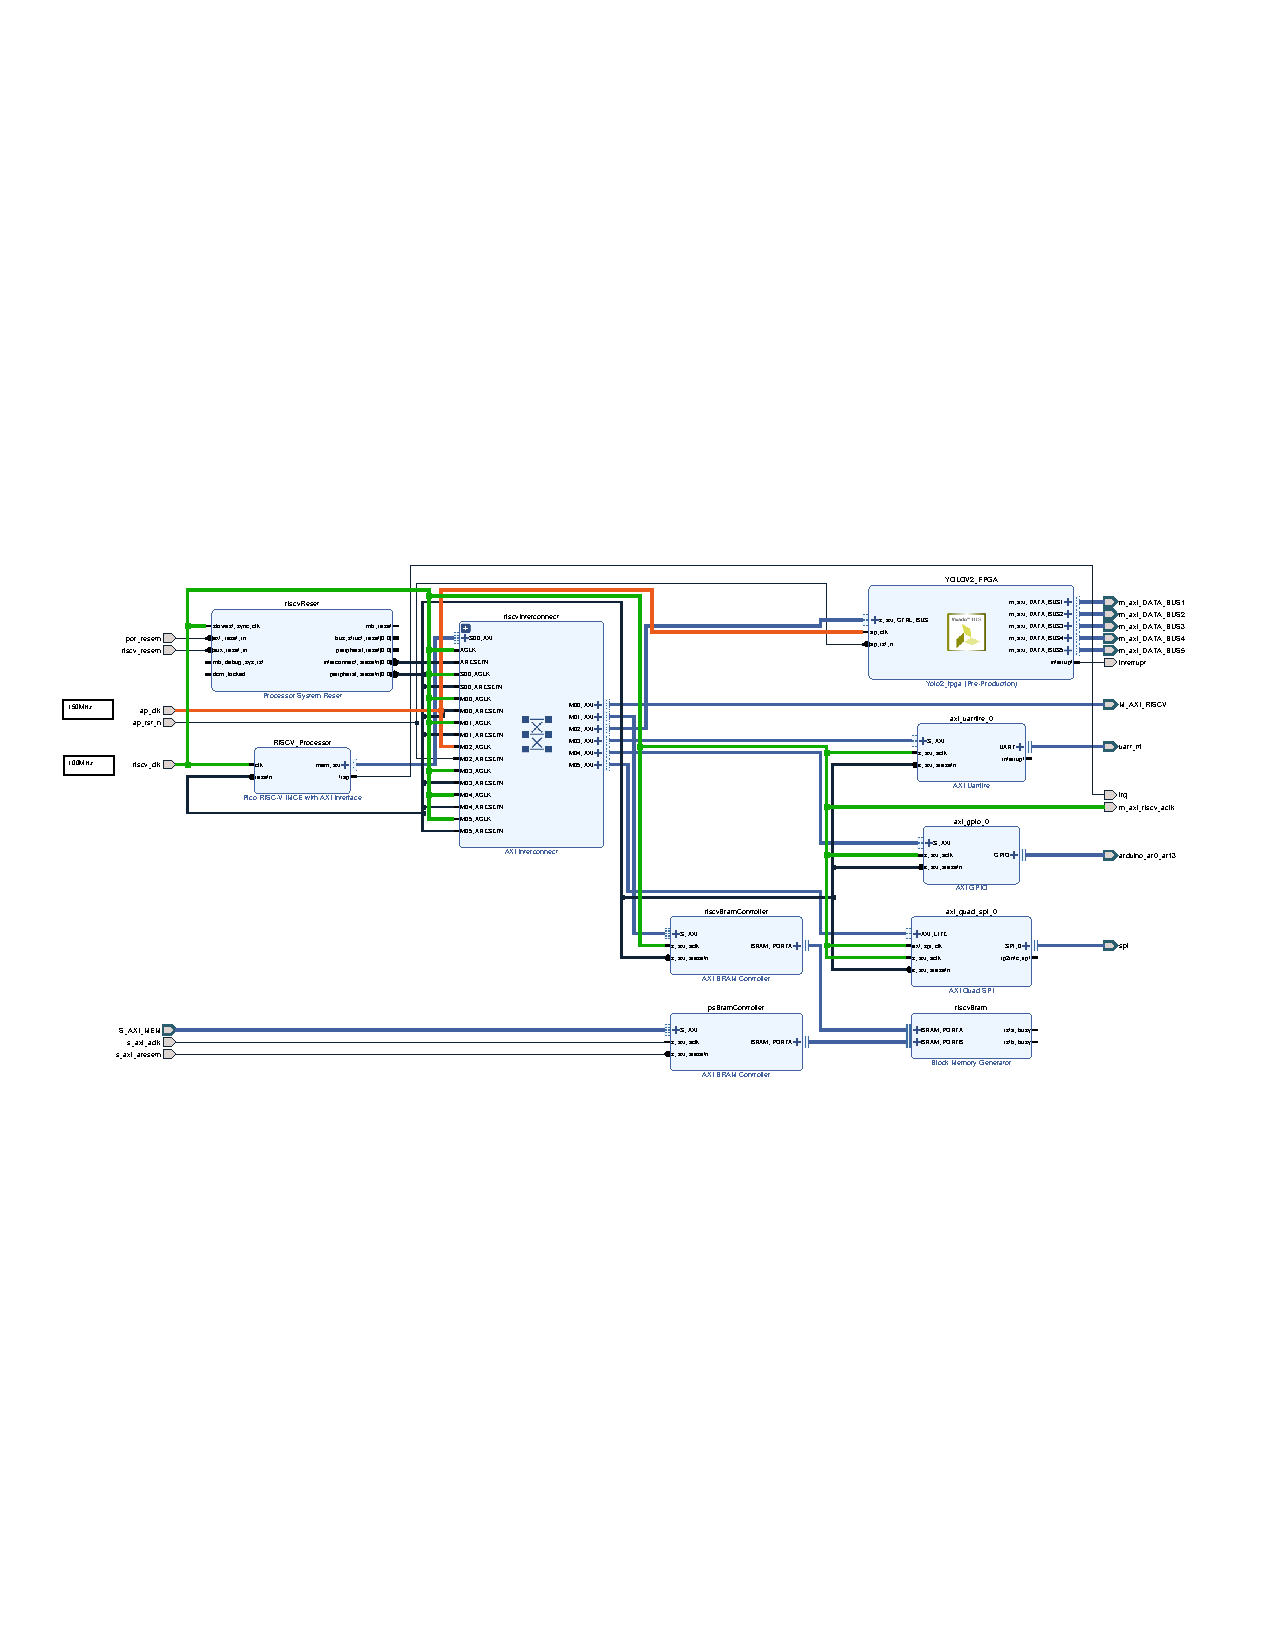
\includegraphics[width=1.0\textwidth,trim=20 270 20 270,clip]{VivadoStructure}
    \caption{异构运算系统}
    \label{fig:VivadoStructure}
\end{figure}

结合设计参数,计算得到 CNN 加速器的预估资源消耗;使用 Vivado 工具综合分别在没有加入 CNN 加速器的情况下和加入了 CNN 加速器的情况下综合硬件工程,在 Vivado 综合布线完成,根据运行报告,将两次消耗的资源相减,获得 CNN 加速器的实际资源消耗。预估资源消耗与实际资源消耗对比如表~\ref{tab:resource}所示:

\begin{table}[!htbp]
\caption{预估资源消耗与实际资源消耗对比}
\label{tab:resource}
\centering
\footnotesize% fontsize
\setlength{\tabcolsep}{4pt}% column separation
\renewcommand{\arraystretch}{1.2}%row space 
\begin{tabular}{lccccc}
\toprule
            & DSP       & BRAM 36Kb& LUT         & FF           & Freq \\
\midrule
Estimate    & 128(58\%) & 85(61\%) & 20736(39\%) & -            & 150MHz \\
Actual      & 153(70\%) & 87(62\%) & 37446(70\%) & 44236(41\%)  & 150MHz \\
\bottomrule
\end{tabular}
\end{table}

DSP 资源主要用于卷积计算模块中的加法器和乘法器的实现,实际消耗的 DSP 资源和预估的相差比较大。由于 HLS 在综合的过程中会考虑到时序状况,当运行频率提高后,HLS 工具会使用更多的 DSP 资源来优化时序,因此实际设计中多出的 DSP 资源消耗主要是用于时序优化的部分。

BRAM 资源主要用于实现 CNN 加速器的缓存以及 AXI 总线接口部分的缓存,实际的 BRAM 资源消耗与预估资源消耗较为接近。

预估资源消耗中的 LUT 是权重数据的缓存所使用的数量,由于 BRAM 的最小值为 18Kb,而权重数据的数据量过小,使用 BRAM 进行缓存较为浪费,因此在本设计中使用 LUT 和 FF 来缓存 权重数据。实际设计 LUT 还要用来实现加速器中的其他模块,难以预估这部分的使用量,因此才产生了 LUT 资源的预估使用量与实际使用量相差较大的现象。

% 由于单个的权重数据缓存的数据量过小($Nky \times Nkx \times Bitwidth = 144b$),无法充分利用 BRAM。因此在设计的过程中,使用 LUT 和 FF 来实现权重数据缓存,在当前设计中,单个权重缓存约消耗 3 个 LUT。因此权重缓存总计消耗 $3 \times Tof_{max} \times Tif_{max} \times 2 = 768$ 个 LUT。与此同时,本设计中,16位定点精度的卷积模块消耗 19968 个 LUT,因此共消耗 20736 个 LUT。实际设计中消耗的 LUT 比预估多出来的那部分是用于实现 CNN 加速器中的其他模块。

\section{CNN 加速器性能评估}

分别测试本设计在 FPGA 平台上实现的 CNN 加速器的性能、CPU 平台 CNN 运算的性能和嵌入式 GPU 平台的上 CNN 运算的性能,进行对比分析。使用单位时间内处理的图片张数(FPS)作为性能对比依据;分析中的功耗为对应芯片的最大功耗。

\subsection{与 CPU 的性能和能效对比}

% 如表~\ref{tab:CompareCPU}所示,与 CPU 相比,本设计中的异构计算系统的能效是四核 ARM A53 的 354.4 倍,i7-9700K 的 120.1 倍;速度是四核 ARM A53 的 361.1 倍,i7-9700K 的 6.3 倍左右。本系统由于硬件资源的限制,计算能力较弱,但是其功耗较低,使得计算产生的时延较长;而 i7-9700K 与其相反,计算能力强,计算的时延很短,但是由于功耗过高,导致其功耗低下。异构系统的功耗虽然略高于四核 ARM A53,但是异构系统的计算时延远优于四核 ARM A53。

本文设计的加速器与 CPU 平台的对比效果如表~\ref{tab:CompareCPU}所示,与 i7-9700K 相比,本文设计的异构计算系统的计算速度是其 6.3 倍;与四核 ARM A53 相比,本文设计的异构计算系统的速度是其 361.1 倍。由对比测试的结果分析可知,X86 架构的主机计算平台计算性能强,计算产生的时延很短,但是由于其功耗过高,导致整体上能效低下;而嵌入式CPU计算平台的计算性能较差,即使功耗较低,其处理图片的速度也是难以接受的;而本文设计的异构计算系统的计算速度优于X86 架构的主机计算平台,且功耗和嵌入式 CPU 平台相近。因此相对于 CPU,本异构计算系统无论在功耗还是计算速度上都有较大的优势。

\begin{table}[!htbp]
\caption{与 CPU 对比}
\label{tab:CompareCPU}
\centering
\footnotesize% fontsize
\setlength{\tabcolsep}{4pt}% column separation
\renewcommand{\arraystretch}{1.2}%row space 
\begin{tabular}{lccc}
\toprule
Device                  & CPU i7-9700K          & Raspberry Pi 3B       & CPU+FPGA \\
\midrule
Technology(nm)          & 14                    & 40                    & 28    \\
Clock(Hz)               & 4.9G                  & 1.2G                  & 666.67M + 150M \\
Memory(MB)              & 32768                 & 1024                  & 512   \\
Max System Power(W)     & 95                    & 5.0                   & 5.0  \\
% Performance(GOP/s)      & 4.11          & 0.27              & 30.15 \\
Latency per img(seconds)& 6.82                  & 390                   & 1.08 \\
FPS($seconds^{-1}$)     & 0.146                 & 0.00256               & 0.926 \\
Power Efficiency(FPS/W) & $1.54 \times 10^{-3}$ & $0.522 \times 10^{-3}$& $185 \times 10^{-3}$ \\
\bottomrule
\end{tabular}
\end{table}

在准确度方面,本文设计的异构计算系统的使用是动态定点 16 位数据量化得到的模型,在准确度上与原模型相近,在 VOC 2007 数据集上 mAP(mean Average Precision)达到了 49.2\%。

\subsection{与嵌入式 GPU 性能与能效对比}

如表~\ref{tab:CompareGPU}所示,与目前常用的的嵌入式 GPU 计算平台相比,由于用于测试的异构计算系统本身的资源较少,导致异构计算系统的算力较低,同时由于工艺制程相差也较大,导致功耗方面也没有优势。文献\citep{nakahara2018lightweight}中提到,在特征提取层使用二值化精度的权重数据,而之后的层使用 32 位精度的浮点数据,可以使加速器更大维度展开,从而在性能上取得更好的效果。

% 但是如文献\citep{nakahara2018lightweight}中所说,如果考虑相同工艺下的 FPGA 芯片,且采用更低的数据精度,则异构平台的性能和功耗上都可以取得较好的效果。

\begin{table}[!htbp]
\caption{与 GPU 对比}
\label{tab:CompareGPU}
\centering
\footnotesize% fontsize
\setlength{\tabcolsep}{4pt}% column separation
\renewcommand{\arraystretch}{1.2}%row space 
\begin{tabular}{lccc}
\toprule
Device & Jetson Nano & CPU+FPGA \\
\midrule
Technology(nm)          & 16    & 28    \\
Clock(Hz)               & 1.43G & 666.67M + 150M \\
Memory(MB)              & 4096  & 512   \\
Max System Power(W)    & 10.0   & 5.0 \\
% Performance(GOP/s)      & 229.89 & 279.99 & 30.15 \\
Latency per img(seconds)& 0.262 & 1.08 \\
FPS($seconds^{-1}$)     & 3.80 & 0.926 \\
Power Efficiency(FPS/W) & 0.380 & 0.185 \\
\bottomrule
\end{tabular}
\end{table}

\section{本章小结}

本章主要计算分析了 CNN 加速器的资源消耗,保证了在使用 HLS 工具进行设计的过程中没有出现重大的资源浪费。根据常见的运算平台,设计了3组典型的对照实验环境,将本设计中的异构计算系统分别与其进行对比,量化分析了该异构计算系统的性能和功耗参数。

\chapter{总结与展望}\label{chap:summary}

% 近年来,卷积神经网络为代表的深度学习算法在许多领域中取得了巨大的突破,如模式识别、图像处理、计算机视觉等。由于 FPGA 低功耗、低延时、可重配置的特性,适合应用于一些对功耗有限制的小型流式应用场景。目前限制 FPGA 在深度学习领域无法大规模应用的主要有以下的两点:

% \begin{enumerate}
%     \item 开发效率低。随着高层次综合技术(HLS)的不断成熟,已经可以使用 C、C++ 等高级语言进行 FPGA 算法开发,该问题正逐步被解决;

%     \item 通用性差,对硬件资源要求高。受制于 FPGA 芯片资源的限制,低成本的 FPGA 芯片往往无法实现一些复杂的算法。
% \end{enumerate}

% 因此本文设计的一种使用 RISC-V 处理器的异构卷积神经网络算法加速系统,将 CNN 网络进行部分展开,展开程度可以根据具体 FPGA 芯片资源的丰富程度灵活调整,同时使用了一个 RISC-V 处理器来完成一些不适合放在 FPGA 上完成的计算任务,在保证了运算速度的提升下,架构的通用性也得到了保证。

% 本课题对使用 FPGA 进行卷积神经网络运算加速做了一定的研究,但由于时间的限制,任然有许多可以进一步研究的地方:

% \begin{enumerate}
%     \item 优化 RISC-V SOC 的设计,将加速器的调用设计成专用指令的形式,进一步提升加速器使用的通用性和便利性;

%     \item 使用多 FPGA 构建大规模协同运行的 CNN 加速网络,使得 CNN 加速的效果不在受限于单个 FPGA 的资源,从而实现一些更复杂的模型;

%     \item 使用 FPGA 的可重构技术,将 CNN 网络进行分片,相当于对局部的 CNN 网络进行了更大维度的展开,从而提升 CNN 网络的并行性,进一步优化加速器的时延。
% \end{enumerate}


目标检测算法在嵌入式领域有着广泛的应用,比如自动驾驶、无人机图像识别等,这些应用场景不仅对准确度和速度有要求,对功耗也有限制。传统的目标检测算法通常运行在高功耗的 GPU 上,并不适合应用在这些低成本低功耗的嵌入式场景中。本文设计了一种运行在 FPGA 上的异构卷积神经网络算法加速系统,将 CNN 网络进行部分展开,展开程度可以根据具体 FPGA 芯片资源的丰富程度灵活调整,同时使用了一个 RISC-V 软核来完成一些不适合在 FPGA 上完成的计算任务。从而实现了在保证准确度的情况下,使用低成本低功耗的嵌入式平台进行目标检测。

本课题对使用 FPGA 进行卷积神经网络运算加速做了一定的研究,但由于时间的限制,任然有许多可以进一步研究的地方:

\begin{enumerate}
    \item 优化 RISC-V SOC 的设计,将加速器的调用设计成专用指令的形式,进一步提升加速器使用的通用性和便利性;

    \item 使用多 FPGA 构建大规模协同运行的 CNN 加速网络,使得 CNN 加速的效果不在受限于单个 FPGA 的资源,从而实现一些更复杂的模型;

    \item 使用 FPGA 的可重构技术,将 CNN 网络进行分片,相当于对局部的 CNN 网络进行了更大维度的展开,从而提升 CNN 网络的并行性,进一步优化加速器的时延。
\end{enumerate}
%---------------------------------------------------------------------------%
% main content

%-
%-> Backmatter: bibliography, glossary, index
%-
\backmatter% initialize the environment
\intotoc*{\cleardoublepage}{\bibname}% add link to toc
{
\begin{spacing}{1.2}           % 参考文献单倍行距
\bibliography{Biblio/ref.bib}% bibliography
\end{spacing}
}
%---------------------------------------------------------------------------%
%->> Backmatter
%---------------------------------------------------------------------------%
\chapter{作者简历及攻读学位期间发表的学术论文与研究成果}

\textbf{本科生无需此部分}。

\section*{作者简历}

\subsection*{casthesis作者}

吴凌云,福建省屏南县人,中国科学院数学与系统科学研究院博士研究生。

\subsection*{ucasthesis作者}

莫晃锐,湖南省湘潭县人,中国科学院力学研究所硕士研究生。

\section*{已发表(或正式接受)的学术论文:}

{
\setlist[enumerate]{}% restore default behavior
\begin{enumerate}[nosep]
    \item ucasthesis: A LaTeX Thesis Template for the University of Chinese Academy of Sciences, 2014.
\end{enumerate}
}

\section*{申请或已获得的专利:}

(无专利时此项不必列出)

\section*{参加的研究项目及获奖情况:}

可以随意添加新的条目或是结构。

\chapter[致谢]{致\quad 谢}\chaptermark{致\quad 谢}% syntax: \chapter[目录]{标题}\chaptermark{页眉}
\thispagestyle{noheaderstyle}% 如果需要移除当前页的页眉
%\pagestyle{noheaderstyle}% 如果需要移除整章的页眉

感激casthesis作者吴凌云学长,gbt7714-bibtex-style
开发者zepinglee,和ctex众多开发者们。若没有他们的辛勤付出和非凡工作,\LaTeX{}菜鸟的我是无法完成此国科大学位论文\LaTeX{}模板ucasthesis的。在\LaTeX{}中的一点一滴的成长源于开源社区的众多优秀资料和教程,在此对所有\LaTeX{}社区的贡献者表示感谢!

ucasthesis国科大学位论文\LaTeX{}模板的最终成型离不开以霍明虹老师和丁云云老师为代表的国科大学位办公室老师们制定的官方指导文件和众多ucasthesis用户的热心测试和耐心反馈,在此对他们的认真付出表示感谢。特别对国科大的赵永明同学的众多有效反馈意见和建议表示感谢,对国科大本科部的陆晴老师和本科部学位办的丁云云老师的细致审核和建议表示感谢。谢谢大家的共同努力和支持,让ucasthesis为国科大学子使用\LaTeX{}撰写学位论文提供便利和高效这一目标成为可能。

\cleardoublepage[plain]% 让文档总是结束于偶数页,可根据需要设定页眉页脚样式,如 [noheaderstyle]
%---------------------------------------------------------------------------%
% other information

%-
%-> Appendix
%-
\mainmatter% initialize the environment
\cleardoublepage%
\appendix% initialize the environment
\chapter{}

\section{\emph{small.spec}}

\lstset{language=C++}
\begin{lstlisting}
#define FEATURE_DATA_TYPE_INT8
#define WEIGHT_DATA_TYPE_INT8
#define WEIGHT_COMPRESSION_DISABLE
#define WINOGRAD_DISABLE 
#define BATCH_DISABLE
#define SECONDARY_MEMIF_DISABLE
#define SDP_LUT_DISABLE
#define SDP_BS_ENABLE
#define SDP_BN_ENABLE
#define SDP_EW_DISABLE
#define BDMA_DISABLE
#define RUBIK_DISABLE
#define RUBIK_CONTRACT_DISABLE
#define RUBIK_RESHAPE_DISABLE
#define PDP_ENABLE
#define CDP_ENABLE
#define RETIMING_DISABLE
#define MAC_ATOMIC_C_SIZE_8
#define MAC_ATOMIC_K_SIZE_8
#define MEMORY_ATOMIC_SIZE_8
#define MAX_BATCH_SIZE_x
#define CBUF_BANK_NUMBER_32
#define CBUF_BANK_WIDTH_8
#define CBUF_BANK_DEPTH_512
#define SDP_BS_THROUGHPUT_1
#define SDP_BN_THROUGHPUT_1
#define SDP_EW_THROUGHPUT_x
#define PDP_THROUGHPUT_1
#define CDP_THROUGHPUT_1
#define PRIMARY_MEMIF_LATENCY_64
#define SECONDARY_MEMIF_LATENCY_x
#define PRIMARY_MEMIF_MAX_BURST_LENGTH_1
#define PRIMARY_MEMIF_WIDTH_64
#define SECONDARY_MEMIF_MAX_BURST_LENGTH_x
#define SECONDARY_MEMIF_WIDTH_x
#define MEM_ADDRESS_WIDTH_32
#define NUM_DMA_READ_CLIENTS_7
#define NUM_DMA_WRITE_CLIENTS_3

#include "projects.spec"

\end{lstlisting}


\section{\emph{Nv\_nvdla\_wrapper.v}}

\lstset{language=Verilog}
\begin{lstlisting}
    NV_NVDLA_apb2csb apb2csb (
        .pclk                  (csb_clk)
        ,.prstn                 (csb_rstn)
        ,.csb2nvdla_ready       (m_csb2nvdla_ready)
        ,.nvdla2csb_data        (m_nvdla2csb_data)
        ,.nvdla2csb_valid       (m_nvdla2csb_valid)
        ,.paddr                 (paddr)
        ,.penable               (penable)
        ,.psel                  (psel)
        ,.pwdata                (pwdata)
        ,.pwrite                (pwrite)
        ,.csb2nvdla_addr        (m_csb2nvdla_addr)
        ,.csb2nvdla_nposted     (m_csb2nvdla_nposted)
        ,.csb2nvdla_valid       (m_csb2nvdla_valid)
        ,.csb2nvdla_wdat        (m_csb2nvdla_wdat)
        ,.csb2nvdla_write       (m_csb2nvdla_write)
        ,.prdata                (prdata)
        ,.pready                (pready)
    );
    NV_nvdla nvdla_top (
        .dla_core_clk                    (core_clk)
        ,.dla_csb_clk                     (csb_clk)
        ,.global_clk_ovr_on               (1'b0)
        ,.tmc2slcg_disable_clock_gating   (1'b0)
        ,.dla_reset_rstn                  (rstn)
        ,.direct_reset_                   (1'b1)
        ,.test_mode                       (1'b0)
        ,.csb2nvdla_valid                 (m_csb2nvdla_valid)
        ,.csb2nvdla_ready                 (m_csb2nvdla_ready)
        ,.csb2nvdla_addr                  (m_csb2nvdla_addr)
        ,.csb2nvdla_wdat                  (m_csb2nvdla_wdat)
        ,.csb2nvdla_write                 (m_csb2nvdla_write)
        ,.csb2nvdla_nposted               (m_csb2nvdla_nposted)
        ,.nvdla2csb_valid                 (m_nvdla2csb_valid)
        ,.nvdla2csb_data                  (m_nvdla2csb_data)
        ,.nvdla2csb_wr_complete           () //FIXME: no such port in apb2csb
        ,.nvdla_core2dbb_aw_awvalid       (nvdla_core2dbb_aw_awvalid)
        ,.nvdla_core2dbb_aw_awready       (nvdla_core2dbb_aw_awready)
        ,.nvdla_core2dbb_aw_awaddr        (nvdla_core2dbb_aw_awaddr)
        ,.nvdla_core2dbb_aw_awid          (nvdla_core2dbb_aw_awid)
        ,.nvdla_core2dbb_aw_awlen         (nvdla_core2dbb_aw_awlen)
        ,.nvdla_core2dbb_w_wvalid         (nvdla_core2dbb_w_wvalid)
        ,.nvdla_core2dbb_w_wready         (nvdla_core2dbb_w_wready)
        ,.nvdla_core2dbb_w_wdata          (nvdla_core2dbb_w_wdata)
        ,.nvdla_core2dbb_w_wstrb          (nvdla_core2dbb_w_wstrb)
        ,.nvdla_core2dbb_w_wlast          (nvdla_core2dbb_w_wlast)
        ,.nvdla_core2dbb_b_bvalid         (nvdla_core2dbb_b_bvalid)
        ,.nvdla_core2dbb_b_bready         (nvdla_core2dbb_b_bready)
        ,.nvdla_core2dbb_b_bid            (nvdla_core2dbb_b_bid)
        ,.nvdla_core2dbb_ar_arvalid       (nvdla_core2dbb_ar_arvalid)
        ,.nvdla_core2dbb_ar_arready       (nvdla_core2dbb_ar_arready)
        ,.nvdla_core2dbb_ar_araddr        (nvdla_core2dbb_ar_araddr)
        ,.nvdla_core2dbb_ar_arid          (nvdla_core2dbb_ar_arid)
        ,.nvdla_core2dbb_ar_arlen         (nvdla_core2dbb_ar_arlen)
        ,.nvdla_core2dbb_r_rvalid         (nvdla_core2dbb_r_rvalid)
        ,.nvdla_core2dbb_r_rready         (nvdla_core2dbb_r_rready)
        ,.nvdla_core2dbb_r_rid            (nvdla_core2dbb_r_rid)
        ,.nvdla_core2dbb_r_rlast          (nvdla_core2dbb_r_rlast)
        ,.nvdla_core2dbb_r_rdata          (nvdla_core2dbb_r_rdata)
        ,.dla_intr                        (dla_intr)
        ,.nvdla_pwrbus_ram_c_pd           (32'b0)
        ,.nvdla_pwrbus_ram_ma_pd          (32'b0)
        ,.nvdla_pwrbus_ram_mb_pd          (32'b0)
        ,.nvdla_pwrbus_ram_p_pd           (32'b0)
        ,.nvdla_pwrbus_ram_o_pd           (32'b0)
        ,.nvdla_pwrbus_ram_a_pd           (32'b0)
    ); // nvdla_top
assign nvdla_core2dbb_aw_awsize = 3'b011;
assign nvdla_core2dbb_ar_arsize = 3'b011;
assign m_axi_awburst = 2'b01;
assign m_axi_awlock  = 1'b0;
assign m_axi_awcache = 4'b0010;
assign m_axi_awprot  = 3'h0;
assign m_axi_awqos   = 4'h0;
assign m_axi_awuser  = 'b1;
assign m_axi_wuser   = 'b0;
assign m_axi_arburst = 2'b01;
assign m_axi_arlock  = 1'b0;
assign m_axi_arcache = 4'b0010;
assign m_axi_arprot  = 3'h0;
assign m_axi_arqos   = 4'h0;
assign m_axi_aruser  = 'b1;
assign pslverr = 1'b0;
endmodule
\end{lstlisting}

\section{\emph{Lenet5 量化关键代码}}

\lstset{language=Python}
\begin{lstlisting}
# Returns a numpy buffer of shape (num_images, 1, 28, 28)
def load_data(filepath):
    test_imgs = []
    global fileList
    fileList = os.listdir(filepath)
    mean = np.ones([3, 224, 224], dtype=np.float)
    mean[0,:,:] = 104
    mean[1,:,:] = 117
    mean[2,:,:] = 123
    for img_path in fileList:
        img_path = filepath +'/'+ img_path
        img = cv.imread(img_path)
        img = crop_img(img, [224, 224])
        img = img.transpose((2, 0, 1))
        img = img - mean
        test_imgs.append(img)
    # Need to scale all values to the range of [0, 1]
    return np.ascontiguousarray(test_imgs).astype(np.float32)

# Returns a numpy buffer of shape (num_images)
def load_labels(filepath):
    global fileList
    test_labels = []
    labels_mapping = {}
    with open(filepath, 'r') as f:
        lines = f.readlines()
        for each in lines:
            imageName, labels = each.strip('\n').split(' ')
            labels_mapping[imageName] = int(labels)
    for each in fileList:
        test_labels.append(labels_mapping[each])
    return np.ascontiguousarray(test_labels)
\end{lstlisting}

\section{\emph{Cache to Json}}

\lstset{language=Python}
\begin{lstlisting}
import json
from collections import OrderedDict
from google.protobuf import text_format
import caffe.proto.caffe_pb2 as caffe_pb2      # 载入caffe.proto编译生成的caffe_pb2文件


caffeprototxt_path = "./deploy.prototxt"
calibletable_json_path = "./resnet18-cifar10-int8.json"
# load deploy.prototxt
net = caffe_pb2.NetParameter()
text_format.Merge(open(caffeprototxt_path).read(), net)
# load jsonfile
with open(calibletable_json_path, "r") as f:
    calible = json.load(f, object_pairs_hook=OrderedDict)
_scales = []
_mins = []
_maxs = []
_offsets = []
_new = OrderedDict()
items = calible.items()
for key, value in items:
    _scales.append(value['scale'])
    _mins.append(value['min'])
    _maxs.append(value['max'])
    _offsets.append(value['offset'])
for idx, _layer in enumerate(net.layer):
    _tempDict =  OrderedDict({
        "scale": _scales[idx],
        "min": _mins[idx],
        "max": _maxs[idx],
        "offset": _offsets[idx],
    }) 
    _new[_layer.name] =_tempDict
with open('resnet18-cifar10-int8-fixed.json', 'w') as f:
    json.dump(_new, f)
\end{lstlisting}

\section{\emph{system-user.dtsi}}

\begin{lstlisting}
/include/ "system-conf.dtsi"
/ {
    reserved-memory {
        #address-cells = <1>;
        #size-cells = <1>;
        ranges;
    
        nvdla_reserved: buffer@0x30000000 {
            compatible = "shared-dma-pool";
            no-map;
            reg = <0x30000000 0x10000000>;
        };
    };
};

&NV_nvdla_wrapper_0{
    compatible = "nvidia,nv_small";
    memory-region = <&nvdla_reserved>;
};
\end{lstlisting}

\section{\emph{Makefile}}

\begin{lstlisting}
obj-m := opendla.o

###append all of sources###
opendla-objs := nvdla_core_callbacks.o nvdla_gem.o scheduler.o engine.o bdma.o conv.o sdp.o cdp.o pdp.o rubik.o cache.o common.o engine_data.o engine_isr.o engine_debug.o
###########################


SRC := $(shell pwd)

all:
    $(MAKE) -C $(KERNEL_SRC) M=$(SRC)

modules_install:
    $(MAKE) -C $(KERNEL_SRC) M=$(SRC) modules_install

clean:
    rm -f *.o *~ core .depend .*.cmd *.ko *.mod.c
    rm -f Module.markers Module.symvers modules.order
    rm -rf .tmp_versions Modules.symvers
\end{lstlisting}

\section{\emph{opendla.bb}}

\begin{lstlisting}
SUMMARY = "Recipe for  build an external opendla Linux kernel module"
SECTION = "PETALINUX/modules"
LICENSE = "GPLv2"
LIC_FILES_CHKSUM = "file://COPYING;md5=12f884d2ae1ff87c09e5b7ccc2c4ca7e"

inherit module

SRC_URI = "file://Makefile \
            file://nvdla_core_callbacks.c \
            file://nvdla_gem.c \
            file://scheduler.c \
            file://engine.c \
            file://bdma.c \
            file://conv.c \
            file://sdp.c \
            file://cdp.c \
            file://pdp.c \
            file://rubik.c \
            file://cache.c \
            file://common.c \
            file://engine_data.c \
            file://engine_isr.c \
            file://engine_debug.c \
            file://common.h \
            file://dla_debug.h \
            file://dla_fw_version.h \
            file://dla_engine.h \
            file://dla_engine_internal.h \
            file://dla_err.h \
            file://dla_interface.h \
            file://dla_sched.h \
            file://engine_debug.h \
            file://nvdla_interface.h \
            file://nvdla_linux.h \
            file://opendla.h \
            file://opendla_initial.h \
            file://opendla_small.h \
            file://nvdla_ioctl.h \
            file://COPYING \
        "
S = "${WORKDIR}"

# The inherit of module.bbclass will automatically name module packages with
# "kernel-module-" prefix as required by the oe-core build environment.
\end{lstlisting}

\section{Lenet5-MNIST.prototxt}
% appendix content

\end{document}
%---------------------------------------------------------------------------%

